\providecommand{\econtexRoot}{..}
% The \commands below are required to allow sharing of the same base code via Github between TeXLive on a local machine and ShareLaTeX.  This is an ugly solution to the requirement that custom LaTeX packages be accessible, and that ShareLaTeX seems to ignore symbolic links (even if they are relative links to valid locations)
\providecommand{\econtex}{./texmf-local/tex/latex/econtex}
\providecommand{\econtexSetup}{./texmf-local/tex/latex/econtexSetup}
\providecommand{\econtexShortcuts}{./texmf-local/tex/latex/econtexShortcuts}
\providecommand{\econtexBibMake}{./texmf-local/tex/latex/econtexBibMake}
\providecommand{\econtexBibStyle}{./texmf-local/bibtex/bst/econtex}
\providecommand{\notes}{./texmf-local/tex/latex/handout}
\providecommand{\handoutSetup}{./texmf-local/tex/latex/handoutSetup}
\providecommand{\handoutShortcuts}{./texmf-local/tex/latex/handoutShortcuts}
\providecommand{\handoutBibMake}{./texmf-local/tex/latex/handoutBibMake}
\providecommand{\handoutBibStyle}{./texmf-local/bibtex/bst/handout}

  

\documentclass[titlepage]{\econtex}

\usepackage{\econtexSetup}\usepackage{\econtexShortcuts}
\providecommand{\texname}{cssUSSaving}
\usepackage{layouts,psfrag,amssymb}
\usepackage{graphicx}
\usepackage{rotating}

\usepackage[compatibility=false]{caption}
\usepackage{subcaption}

\usepackage[T1]{fontenc}
\usepackage{lmodern}



\definecolor{jirkasblue}{rgb}{0.2,0.2,0.7}
\definecolor{Cerulean}{rgb}{0,0.48,0.652}
\definecolor{Purple}{rgb}{0.5,0,0.5}
\definecolor{Lime}{rgb}{0.52,0.706,0}
\definecolor{Red}{rgb}{1,0,0}

\newcommand{\jemph}[1]{{\color{Red}#1}}
\newcommand{\bemph}[1]{{\color{jirkasblue}#1}}
\newcommand{\jbemph}[1]{{\textbf{\color{jirkasblue}#1}}}



\provideboolean{ifWeb}
\setboolean{ifWeb}{false}
\ifdvi{\setboolean{ifWeb}{true}}\fi
\opt{Web}{\setboolean{ifWeb}{true}}

\ifthenelse{\boolean{ifWeb}}{\usepackage{grfext}
\PrependGraphicsExtensions*{.svg,.SFG,.jpg,.JPG,.png,.PNG,.pdf,.PDF}
}{}


\opt{EndFloats}{\RequirePackage[noheads,nolists,tablesfirst,nomarkers]{endfloat}\renewcommand{\efloatseparator}{\mbox{}}}

\hypersetup{pdfauthor={Christopher Carroll <ccarroll@jhu.edu>, Jiri Slacalek <jiri.slacalek@ecb.europa.eu>, Martin Sommer <msommer@imf.org>},
            pdfsubject={Dissecting Saving Dynamics: Measuring Credit, Wealth and Precautionary Effects},
            pdfkeywords={Consumption, Saving, Wealth, Credit Availability, Uncertainty; JEL: E21, E32
            },
            pdfproducer = {LaTeX with hyperref and thumbpdf},
            pdfcreator = {ps2pdf, pdfwrite}
            }

\definecolor{Cerulean}{rgb}{0,0.48,0.652}
\DeclareMathOperator*{\argmin}{arg\,min}

\begin{document}\bibliographystyle{\econtexBibStyle}
\hfill{\tiny \texname, \today}

\begin{verbatimwrite}{\texname.title}
Dissecting Saving Dynamics: Measuring Wealth, Precautionary, and Credit Effects
\end{verbatimwrite}

\title{Dissecting Saving Dynamics:  Measuring Wealth, Precautionary, and Credit Effects  }

\medskip\medskip

\author{
{Christopher Carroll\tiny{~}}\authNum \\ {\small JHU}
\and
{Jiri Slacalek\tiny{~}}\authNum \\ {\small ECB}
\and
{Martin Sommer\tiny{~}}\authNum \\ {\small IMF}
}

\date{April 29, 2019}

\maketitle


\keywords{Consumption, Saving, Wealth, Credit, Uncertainty}
\jelclass{E21, E32}


\begin{abstract}\ifthenelse{\boolean{ifWeb}}{\Large \hypertarget{abstract}{}}{}
We show that an estimated tractable `buffer stock saving' model can match the 30-year decline in the U.S.\ saving rate leading up to 2007, the sharp increase during the Great Recession, and much of the intervening business cycle variation.  Saving depends on the gap between `target' and actual wealth, with the target determined by measured credit availability and measured uncertainty.  Following financial deregulation starting in the late 1970s, expanding credit supply explains the trend decline in saving, while fluctuations in wealth and consumer-survey unemployment expectations capture the business-cycle variation, including the sharp rise during the Great Recession.
\ifthenelse{\boolean{ifWeb}}{\Large}{}
\end{abstract}

\parbox{\textwidth}{
\begin{center}
\begin{tabbing}
\texttt{Archive:~} \= \= \url{http://econ.jhu.edu/people/ccarroll/papers/cssUSSaving.pdf} \kill \\  
\texttt{~~~~Web:~} \> \> \url{http://econ.jhu.edu/people/ccarroll/papers/cssUSSaving/} \\
\texttt{~~~~PDF:~} \> \> \url{http://econ.jhu.edu/people/ccarroll/papers/cssUSSaving.pdf} \\
\texttt{~Slides:~} \> \> \url{http://econ.jhu.edu/people/ccarroll/papers/cssUSSaving-Slides.pdf} \\
\texttt{~~~Repo:~} \> \> \url{https://github.com/llorracc/cssUSSaving} \\
\texttt{~~~~~~~~~} \> \> {\it (Contains data and estimation software producing paper's results)}
\end{tabbing}
\end{center}
}

\begin{authorsinfo}
\name{Carroll: \href{mailto:ccarroll@jhu.edu}{\texttt{ccarroll@jhu.edu}}, Department of Economics, 
Johns Hopkins University, %Baltimore, MD 21218,
\url{http://econ.jhu.edu/people/ccarroll/}, and National Bureau of Economic Research.}
\name{Slacalek: \href{mailto:jiri.slacalek@ecb.europa.eu}{\texttt{jiri.slacalek@ecb.europa.eu}}, European Central Bank, Frankfurt am Main, Germany, \url{http://www.slacalek.com/}. }
\name{Sommer: \href{mailto:msommer@imf.org}{\texttt{msommer@imf.org}}, International Monetary Fund, Washington, DC, \url{http://martinsommeronline.googlepages.com/}.}
\end{authorsinfo}

\thanks{We thank Andra Buca, Kerstin Holzheu, Geoffrey Keim, Jakub Ryb\'ak, Camilla Sacca and Joanna S{\l}awatyniec for excellent research assistance, and Ricardo Reis, John Duca, Karen Dynan, Robert Gordon, Bob Hall, Mathias Hoffmann, Charles Kramer, David Laibson, Mar\'\i a Luengo-Prado, Bartosz Ma\'ckowiak, John Muellbauer, Valerie Ramey, David Robinson, Damiano Sandri and Jonathan Wright for insightful comments. We are grateful to Abdul Abiad, John Duca, John Muellbauer and Anthony Murphy for sharing their data. The views presented in this paper are those of the authors, and should not be attributed to the International Monetary Fund, its Executive Board, or management, or to the European Central Bank.}

\titlepagefinish


\setcounter{page}{1}

\hypertarget{PRSintro}{}
\begin{figure}
\caption{US Personal Saving Rate (`PSR')}
\label{fig:PSR}
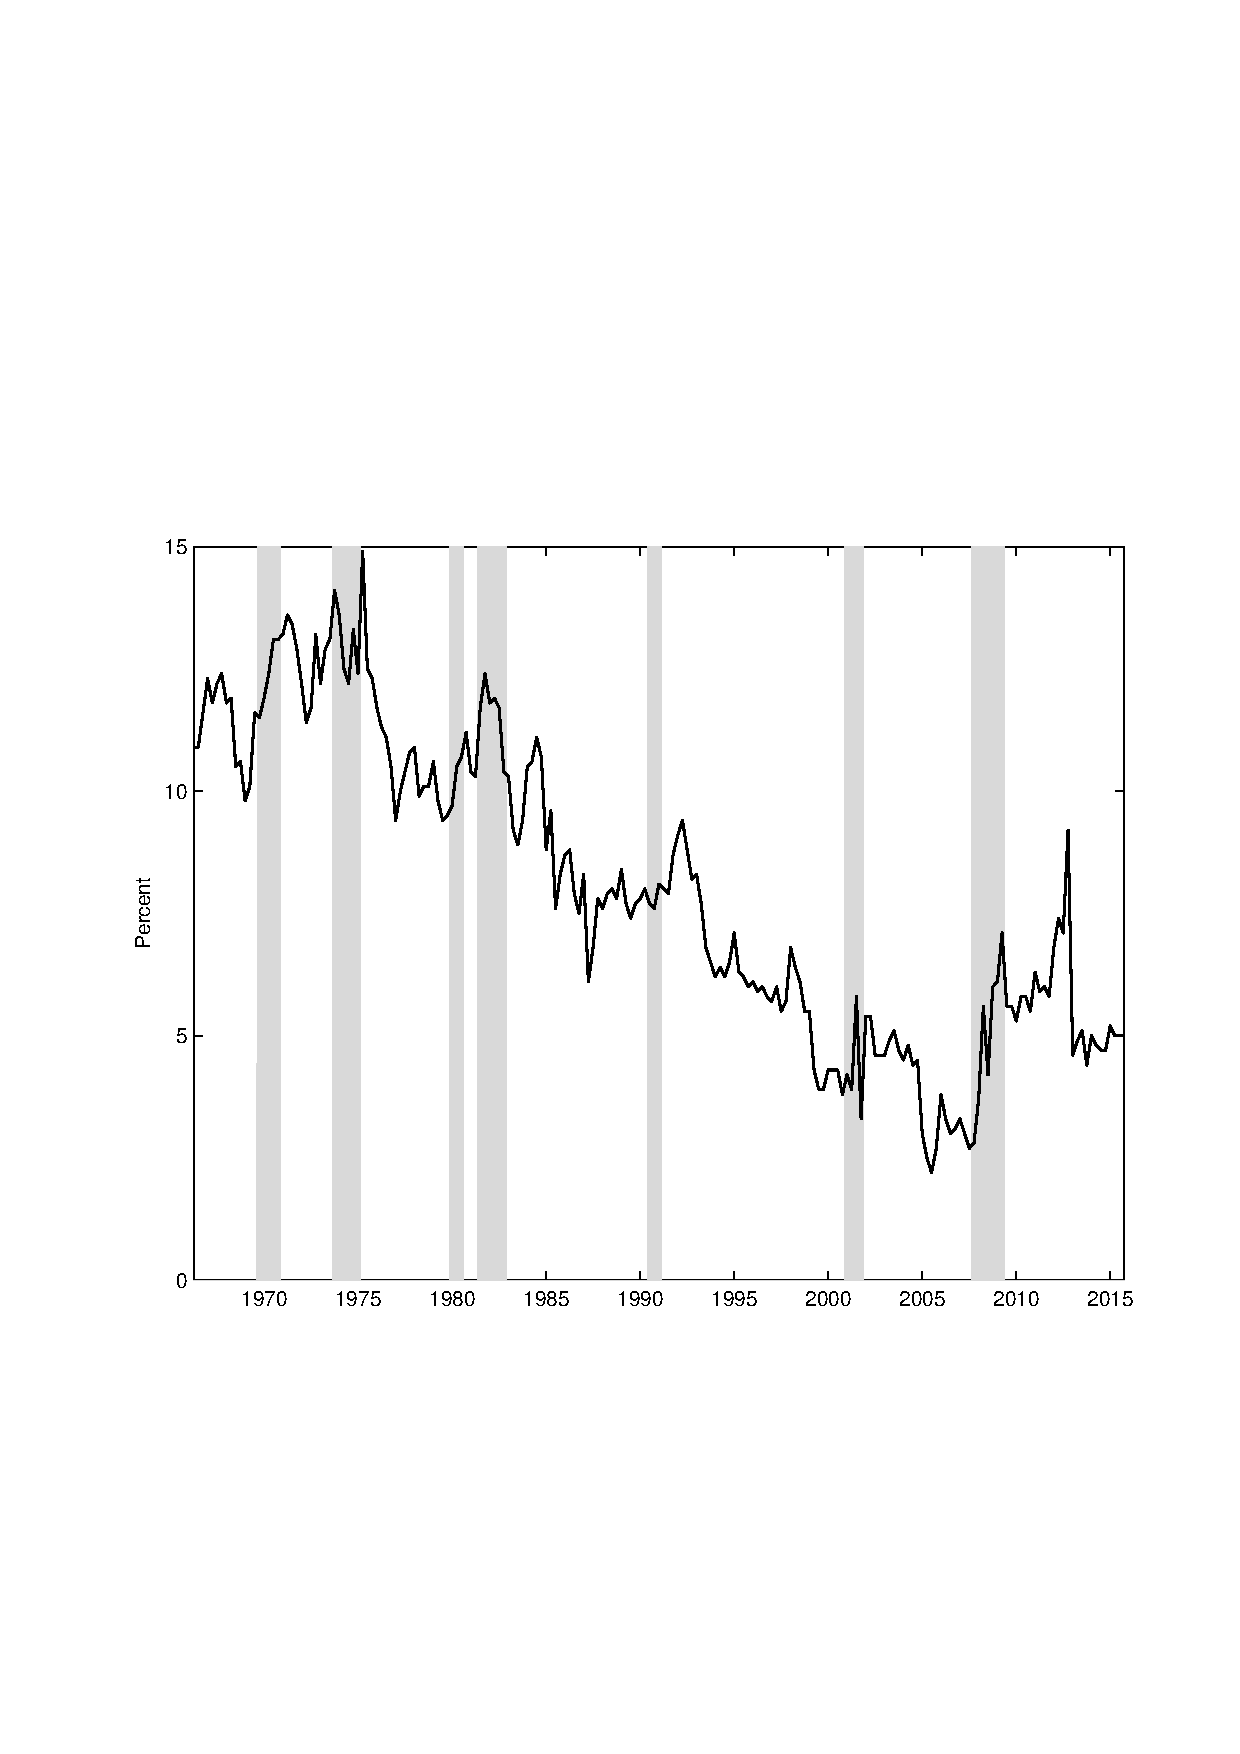
\includegraphics[width=.5\textwidth, height=6.5cm]{\econtexRoot/Figures/fPSR-actual}
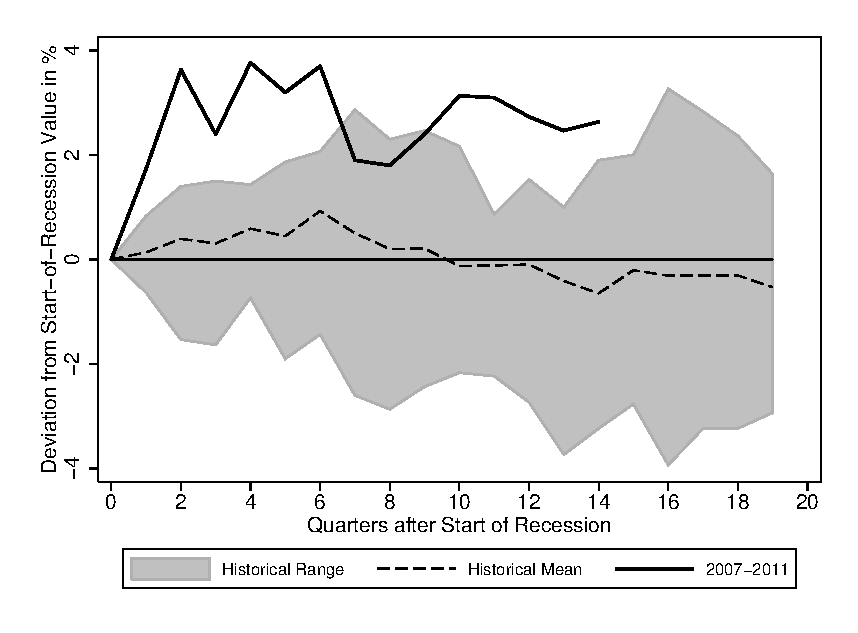
\includegraphics[width=.5\textwidth, height=6.5cm]{\econtexRoot/Figures/saving}

\footnotesize Notes: The left panel shows the personal saving rate, 1966q1--2015q4. The right panel shows the deviation of the saving rate from its value at the start of recessions (in percentage points), over a historical range that includes all recessions after 1960q1. Source: BEA.
\end{figure}



\section{Introduction}

The start of the Great Recession marked a striking break in the behavior of the US personal saving rate. After gradually declining over the previous 30 years, the saving rate doubled during the recession  (Figure~\ref{fig:PSR}(a)), and even 5 years later, exceeded its pre-crisis level by some 4 percentage points (Figure~\ref{fig:PSR}(b)).  Surprising weakness of consumption growth (relative to income growth) was  a key element in explanations of why, year after year, the recovery was weaker than forecasters expected.  The ``secular stagnation'' hypothesis of \cite{summersSecStagReuters,summersSecStagAER}, \cite{krugmanSecStagNYT,krugmanSecStagCEPR}, \cite{gordonSecStag} and others is the most provocative interpretation, but even secular stagnation skeptics have acknowledged that surprisingly weak consumption growth played a role in the anemic recovery (\cite{hhhwSecStagNo}).

Standard consumption models incorporate several mechanisms that interact with income dynamics to generate the saving rate; the channels that have received the most attention include `wealth effects,' the availability of credit, and precautionary motives.\footnote{The literature is large; see among many others the analyses of \cite{carroll:brookings} on precautionary saving during recessions, \cite{cos11}, \cite{mrsBalance}, \cite{BergerEtAl:HPandC} and others on wealth effects, and \cite{mue07} and \cite{parker_nberma_spendthrift} on credit availability and financial liberalization. Some work (e.g., \cite{hall:slump}, \cite{gkLiq}, \cite{glLiq}) has argued (though without much attempt at quantification) that a
sudden sharp reversal of the credit-loosening trend played a large role in the recent saving rise.
Finally, a series of recent papers investigates the role of housing for the dynamics of consumption  (e.g., \cite{justPrimTamb:CredSupplyAndHouseBoom}, \cite{huoRRfinFrictionsGR}, \cite{garrigaHedlund}, \cite{kmv:houseBoomBust} and \cite{goreaMidriganLiqConstraints}), but this work focusses on the dynamics during the global financial crisis (rather than also covering `normal' recessions over the last several decades, as we do). \label{foot:PSRlit}}  But we are not aware of any work that has systematically attempted to quantify the relative importance of these channels using the full (secular and cyclical) variation in the available historical data.  Our contribution is to use a simple structural model of saving to construct such a quantitative decomposition.  Specifically, we estimate a tractable `buffer stock saving' model (an extended version of \cite{ctDiscrete}) with explicit and transparent roles for the three factors emphasized above (the wealth, credit, and precautionary channels). The model's key intuition is that, in the presence of income uncertainty, optimizing households have a target ratio of wealth to permanent income that depends on the usual theoretical considerations (risk aversion, time preference, etc.) and on two features that have been harder to incorporate into analytical models: The degree of labor income uncertainty and the availability of credit.

The structural model is able to capture the bulk of the variation in the saving rate over the historical period for which the necessary data are available---with a fit better than 0.90 in the $R^2$ sense. We find a statistically significant and economically important role for all three explanatory variables. The trend decline in saving between the mid-1970s and 2007 is explained by the continual easing of credit availability during the extended period of gradual financial deregulation that began in the Carter administration (see \cite{wooleyDeregulation} for the history) and extended to the brink of the Great Recession. Our measure of credit supply (based on the Fed's Survey of Senior Loan Officers) shows a substantial tightening during the Great Recession, the first sustained curtailment since the 1970s; but according to the model's estimates, a larger contributor to the sharp increase in the saving rate during the Great Recession was the collapse in household wealth, with an increased precautionary motive (proxied by a measure of consumers' unemployment expectations) also playing a substantial role.\footnote{We treat the three driving variables as exogenous inputs into our partial equilibrium model.  This is unsatisfying, because all three variables are to some degree endogenous to deeper forces; in particular, the collapse in asset prices in the Great Recession is presumably at least partly attributable to the increase in uncertainty and perhaps to the credit tightening.  If there were anything approaching a consensus about the appropriate way to endogenize asset prices (of stocks and, more recently, of housing) we would have preferred to do so, but no such consensus has emerged (see, e.g., the work we refer to in footnotes~\ref{foot:PSRlit} and~\ref{foot_housingLit} for an overview). In this choice, we follow many papers (including \cite{landvoigt:rfs} and recently \cite{krusell:usWealthDistr}), who model asset returns as exogenous (on exogeneity of asset prices see also our discussion in section~\ref{ssAltModels}).
\hypertarget{Exogeneity}{}
}

The rest of the paper is organized as follows. Section~\ref{ssTractableBS} presents the structural model and its mechanics. Section~\ref{DataAndMeasurement} briefly describes the main data; section~\ref{sStructuralEstimation} presents the estimates of the model and the empirical decomposition of the saving rate. Section~\ref{sReducedFormRegressions} compares our framework to the key competing frameworks for thinking about the saving rate; section~\ref{conclusions} concludes.

\hypertarget{ssTractableBS}{}

\section{Theory: Target Wealth and Credit Conditions} \label{ssTractableBS}

Here we introduce the model that we will later estimate, a simple representative-consumer buffer-stock saving model derived from \cite{ctDiscrete} (henceforth CT).  We extend the CT model to incorporate unemployment insurance, which gives the model a mechanism to capture changes in credit availability (because borrowing is assumed to be limited by the minimum possible income available to repay it).

\subsection{Essentials of the Tractable Model}

Under most specifications of uncertainty, Constant Relative Risk Aversion utility interacts with uncertainty in ways that rule out any transparent analytical formulation of the forces at work.

The assumption that makes the CT model tractable despite its use of CRRA utility is that unemployment risk takes a particularly stark form: Employed consumers face a constant probability $\mho$ of becoming unemployed, and, once unemployed, can never become employed again.  The sense in which the model is tractable is that there is a closed form solution for the level of target wealth, and the full consumption function (though numerical) can be derived almost instantaneously from a simple difference equation.  %\footnote{While the unemployment risk in \cite{ctDiscrete} is of a simple form, the key mechanisms at work are the same as those in more sophisticated setups with a realistic specification of uninsurable risks (building on the work of %\cite{bewley:pih}, %\cite{skinner_jme88}, \cite{zeldes_qje89}, \cite{deaton_ecta91}, %\cite{carroll:brookings}, \cite{carroll_bufferStockSaving_qje97} and 

CT show that for the special case of logarithmic utility, the target `market resources' ratio for an employed consumer (roughly, spendable wealth; details below) is:
\begin{eqnarray}
  \mTarg^{e}
  & \approx &
  1 + \left(\frac{1}{(\pGro-\rfree)+\timeRate(1+(\pGro+\timeRate-\rfree)/\urate)}\right),
\label{eq:mTargetLogCase}
\end{eqnarray}
where $\pGro$ is the growth rate of labor income, $\rfree$ is the interest rate and $\timeRate=-\log \DiscFac$ is the time preference rate.

A ``Growth Impatience Condition'' guarantees that the expression $(\pGro+\timeRate-\rfree)$ in the denominator is strictly positive.  Using this fact, the equation has intuitive implications:  Target wealth is higher (the consumer saves more) when
\begin{itemize}
\item The consumer is more patient  (the time preference rate $\timeRate$ is lower)
  \item Unemployment risk $\mho$ is higher (inducing a stronger precautionary motive)
\item (Discounted) future income is lower (that is, $\pGro-\rfree$ is smaller)
  \end{itemize}

  %Large literatures have examined the separate and the joint effects of $\rfree$ and $\pGro$, and have consistently failed to find robust and reproducible results about the relationship between these variables and the saving rate that hold in the short and long run.  Our model does not have much new to say on that subject, so we will follow \cite{cmModel} and many subsequent papers in assuming constant $\rfree$ and $\pGro$.

  \hypertarget{Determinants-of-Target-Wealth}{}

\subsection{Determinants of Target Wealth} \label{ssCfunction}

Our only modification to the CT model is addition of an `unemployment insurance' (UI) system that relaxes the natural borrowing constraint. %\footnote{For the derivations, see online appendix~\ref{apdxUIa}.}
 In the CT model, the necessity of arriving in the unemployment state with some minimal positive level of assets (to prevent zero consumption) induces a `natural borrowing constraint.'  The introduction of UI benefits shifts the consumption function of an employed consumer to the left because households with little market resources are willing to borrow, knowing that they will not starve even if they become unemployed. Consumers will limit their indebtedness, however, to an amount small enough to guarantee that consumption will remain strictly positive even when unemployed (the `natural borrowing constraint' shifts).%\footnote{We could easily add a tighter `artificial' liquidity constraint, imposed exogenously by the financial system, that would prevent the consumers from borrowing as much as the natural borrowing constraint permits.  But \cite{carroll:atheoryjep} shows that the effects of tightening an artificial constraint are qualitatively and quantitatively similar to the effects of tightening the natural borrowing constraint. %We describe the extension of the CT model for the unemployment insurance in an online appendix.
 

 The budget constraint depends on the consumer's employment status. %JS0415 I want to signal in the first sentence that the paragraph is about the budget constraint
  We denote  with lower-case $m$ and $c$ the levels of market resources $M$ (market wealth plus current income) and consumption $C$ normalized by the corresponding period's pretax labor income $\ell\,\Wage$ (the product of individual labor productivity $\ell$ and the aggregate wage $\Wage$); $\ell\,\Wage$ grows by $\PGro=1+\pGro$ per period.  Next period's market resources ratio $m_{t+1}$ is the sum of current market resources $m_{t}$ net of consumption $c_t$, augmented by the (growth-adjusted) interest factor $\Rfree/\PGro$ and income. For the employed consumer (normalized) after-tax labor income is $1-\TaxUI$, while for the unemployed consumer the unemployment benefit is $\Severance$ (both expressed as a fraction labor income). The unemployment benefit $\Severance$ is financed on a pay-as-you-go basis by a lump sum tax $\TaxUI$.  Under these assumptions the (normalized) dynamic budget constraint is:
\begin{equation}
    m_{t+1}=\left\{
    \begin{array}{ll}
    (m_{t}-c_t)\Rfree/\PGro+\Severance & \mbox{with prob. }\phantom{1-~}\urate \quad \text{          (unemployed in $t+1$)}\\
    (m_{t}-c_t)\Rfree/\PGro+1-\TaxUI  & \mbox{with prob. }1-\urate           \quad \text{\phantom{un}(employed in $t+1$)}
    \end{array}
  \right. \label{eq:dbc}
\end{equation} %\medskip

Generalizing  formula \eqref{eq:mTargetLogCase} for relative risk aversion $\CRRA > 1$ and allowing for UI benefits~$\Severance$, the employed consumer's target market resources ratio $\mTarg^{e}$ can be written as a function characterized by:\footnote{%
  Specifically, in online appendix~\ref{apdxUIa} we show that the steady-state target wealth is:
$$
\mTarg^{e}=\frac{(\eta+1)(1-\urate\Severance)-\eta\Severance}{\eta+1-\Rfree/\PGro},
$$
where $\eta=\MPC^u\Pi\Rfree/\PGro$, $\Pi=\Big(\frac{\PGro^\CRRA(\Rfree\DiscFac)^{-1}-(1-\urate)}{\urate}\Big)^{1/\CRRA}$ and $\MPC^u$ is the (constant) marginal propensity to consume out of total wealth for the unemployed consumer. The relationship holds under our estimated parameter values; some of these relationships do not hold for all parameter values.
}
\begin{equation}
\mTarg^{e}=f\big(\mathop{\mho}_{(+)},\mathop{\CEA(\Severance)}_{(-)},\mathop{\Rfree}_{(+)},\mathop{\PGro}_{(-)},\mathop{\CRRA}_{(+)},\mathop{\DiscFac}_{(+)},\dots\big). \label{mTargetNonlin}
\end{equation}
The target wealth $\mTarg^{e}$ increases with unemployment risk $\mho$, as consumers build up a larger precautionary buffer of savings. %\footnote{The increase in $\mho$ is a pure increase in risk (a mean-preserving spread in human wealth) because we assume that labor productivity $\ell$ grows at the rate $1/(1-\mho)$ (which in turn implies that labor income grows at the rate $\PGro=\WGro/(1-\urate)$, where $\WGro$ is the growth rate of the wage $\Wage$).}
An easing of credit conditions (which we denote as `$\CEA$')---an increase in the $\CEA$ index (modelled as an increase in $\Severance$)---allows households to borrow more and thus reduces the need to accumulate wealth for consumption smoothing. A higher interest rate $\Rfree$ increases the rewards to holding wealth and thus increases the amount held. Faster expected growth of labor income $\PGro$ translates into a lower wealth target because optimists consume more now in anticipation of their future prosperity (the `human wealth effect'). Increasing risk aversion $\CRRA$ raises target wealth in a way that is qualitatively similar to the effects of an increase in uncertainty.  And of course, making the consumer more patient (increasing $\DiscFac$) increases target wealth.\footnote{Our final modeling assumption is that we can capture most of the variation in the saving rate by considering the behavior of an economy populated by a single `employed' agent (who is always afraid of becoming unemployed but never does).  (\cite{cjSOE} show that the simulated behavior of an economy populated by a continuum of agents who draw unemployment shocks as specified in the model -- so that at any given time there is a population of employed and of unemployed consumers -- is very well represented by the behavior of the `representative employed consumer' we use here).
}

\subsection{The Three Channels: A Graphical Exposition} \label{ss3channels}


\hypertarget{PhaseDiag}{}

\begin{sidewaysfigure}	\caption{Consumption/Saving Dynamics in a Simple Buffer Stock Model}
	\centering
	\begin{subfigure}[t]{0.49\textheight}
		\centering
    %\addtocounter{figure}{-1}
		{ 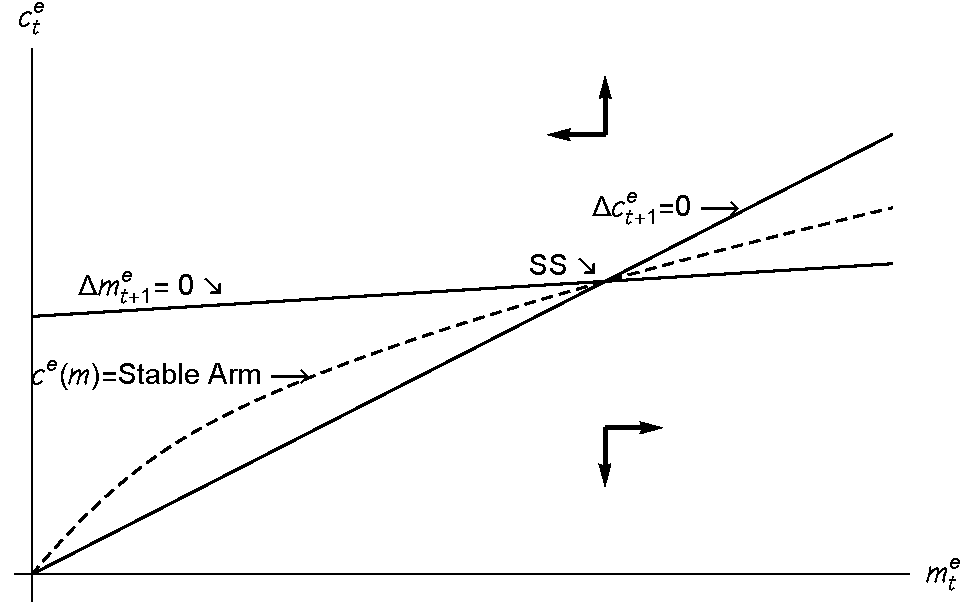
\includegraphics[width=0.49\textheight]{\econtexRoot/Figures/TractableBufferStockPhaseDiag}}
		\caption{Consumption Function (Stable Arm of Phase Diagram)}		\label{fig:PhaseDiag}
	\end{subfigure}
	\begin{subfigure}[t]{0.49\textheight}
		\centering
		{ 
\includegraphics[width=0.49\textheight]{\econtexRoot/Figures/WealthShock}}
		\caption{A Wealth Shock}\label{fig:WealthShock}
	\end{subfigure} \\
	\begin{subfigure}[t]{0.49\textheight}
		\centering
		{ 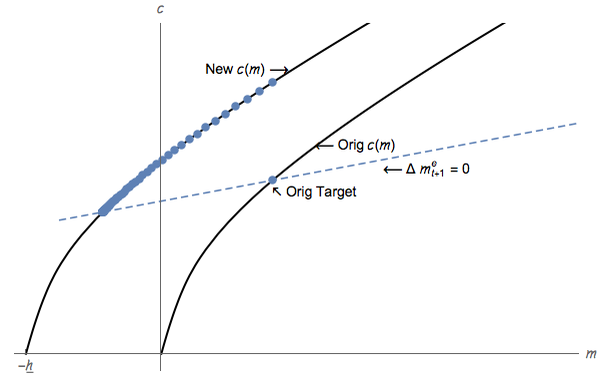
\includegraphics[width=0.49\textheight]{\econtexRoot/Figures/PhaseDiagramDebtLimRisePlot}}
		\caption{Relaxation of Natural Borrowing Constraint from 0 to $\underline{h}$}	\label{fig:PhaseDiagramDebtLimRise}	
	\end{subfigure}
	\begin{subfigure}[t]{0.49\textheight}
		\centering
		{ 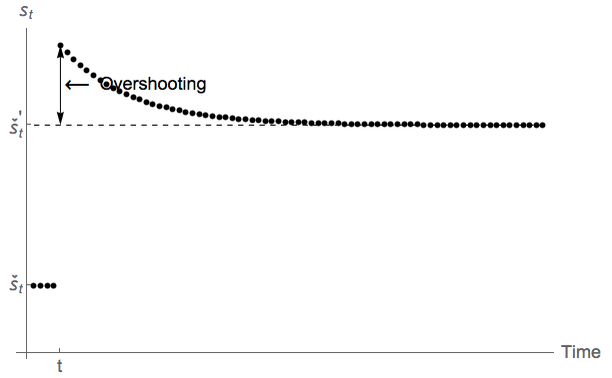
\includegraphics[width=0.49\textheight]{\econtexRoot/Figures/savRateAfterMhoRisePlot}}
		\caption{Saving After an Increase in Uncertainty $\urate$} \label{fig:savRateAfterMhoRisePlot}
\end{subfigure}
\end{sidewaysfigure}


Figure~\ref{fig:PhaseDiag} shows the phase diagram for the CT model.  The (concave) consumption function is indicated by the thick solid locus, which is the saddle path that leads to the steady state (at which  both consumption and market resources, $c$ and $m$, are constant).  Because the precautionary motive diminishes as wealth rises, the model says the saving rate is a declining function of market resources, an implication of consumption concavity. %And, since an expansion in the availability of credit reduces the target level of wealth (and permits an immediate boost to consumption), looser credit conditions lead to lower steady-state saving (and an even greater decline in the saving rate immediately after the credit expansion).

This consumption function can be used directly to analyze the effects of the three channels affecting the saving rate.  For a consumer who starts with market resources equal to the target, $\mRat_{t}=\mTarg^{e}$, the consequences of a pure negative shock to wealth, depicted in Figure~\ref{fig:WealthShock}, are straightforward: Consumption declines upon impact, to a level below the value that would leave $m$ constant (the leftmost red dot); because consumption is below permanent income, $m$ (and thus $c$) rises over time back toward the original target (the sequence of dots).

From an initial borrowing limit of 0 that requires wealth to be positive ($m$ must be strictly greater than $c$), an expansion of unemployment benefits results in a more generous natural borrowing limit $\underline{h}$ (implying minimum net worth of $-\underline{h}<0$) and leads to an immediate increase in consumption for a given level of resources (Figure~\ref{fig:PhaseDiagramDebtLimRise}).  But over time, the higher spending causes the consumer's level of wealth to decline, forcing a corresponding gradual decline in consumption until wealth eventually settles at its new, lower target level.\footnote{Our setup thus reproduces the standard result from the literature on the effects of borrowing constraints; see, e.g., \cite{carroll:atheoryjep}, \cite{mue07}, \cite{glLiq} and \cite{hall:slump}.}

Figure~\ref{fig:savRateAfterMhoRisePlot} shows the consequences of a permanent increase in unemployment risk $\urate$ for the dynamics of the personal saving rate (`PSR' henceforth), rather than the level of consumption (as shown before).  Qualitatively, the effects of a human-wealth-preserving spread in risk are essentially the opposite of a credit loosening: On impact, the PSR jumps upward, overshooting the new target $\check{s}'$ (cf. \cite{dornbuschOvershooting}), followed by a gradual decline toward $\check{s}'$ (which is higher than the original $\check{s}$). This nonmonotonic adjustment of saving to shocks reflects the fact that, when the target level of wealth rises, not only is a higher level of steady-state saving needed to maintain a higher target level of wealth, an immediate \textit{further} boost to saving is necessary to move from the current (inadequate) level of wealth up to the new (higher) target.

\hypertarget{ssAltModels}{}\hypertarget{Comparison-with-Alternative-Frameworks}{}

\subsection{Comparison to Alternative `Structural' Models} \label{ssAltModels}


\begin{verbatimwrite}{./Highlighted/Comparison-with-Alternative-Frameworks.tex}

We use this simple, partial-equilibrium framework (instead of a richer but less tractable HA-GE model) because our goal is to estimate a unified structural saving model whose ``deep'' parameters are jointly identified using both business-cycle-frequency fluctuations AND long-term trends.  Both cyclical and secular changes in the saving rate have been large, and a model that matched one set of facts (secular, or cyclical) but had strongly counterfactual implications for the other would not be a satisfying description of history.

We are not aware of prior papers that attempt this.  Essentially all of the ``structural'' literature has focused on cyclical dynamics, using one of two frameworks:
\begin{enumerate}
\item Complex Heterogeneous Agent New Keynesian models (HANK) with serious treatments of uncertainty
    \item Simple spender--saver Two-Agent New Keynesian models (TANK)
\end{enumerate}



\hypertarget{HA-Model-Too-Hard-Right-Now}{}
\hypertarget{HA-Models-Not-Used-Yet-For-Forecasting}{}
For the first class of models, the last decade or so has seen impressive progress in the degree of realism achievable in the treatment of uncertainty, liquidity constraints, household structure, and other first-order elements of households' microeconomic environment. A flourishing literature today 
explores the implications of these complexities for many questions; see \cite{kmpHandbook} for a survey.
However, at the current state of the art, estimating such a model would be a considerable challenge, as estimation is generally several orders of magnitude more computationally demanding than simulating a calibrated version (which is what the existing literature has done).  Furthermore, rich microfounded models have usually been optimized for the specialized purposes of examining in great depth a single question (such as the mechanisms of transmission of monetary policy, \cite{kmvHANK}) rather than, as we are attempting, to address a number of different causal mechanisms, over different time horizons, simultaneously.  Finally, even if such a rich HA-GE model could be estimated, it is not clear that the extra microeconomic realism would be worth the cost in transparency and tractability.

Indeed, in advocating the use of TANK models, \cite{dgTANK} argue that the simplicity and transparency of models with only two agents more than make up for their lack of fidelity to microeconomic facts.  This point is illustrated by the fact that central banks and other entities that require a theoretical model regularly use TANK models as practical tools for real-time macroeconomic analysis and forecasting. However, a major drawback of the TANK models is that they allow no role for uncertainty either as an impulse or a propagation mechanism, despite the large literature in recent years that has argued the uncertainty is a core element of business cycle dynamics (see, e.g., cf \cite{bfjstUncertain}).

Our  model occupies a middle ground. There is only a single agent (making it simpler in that respect even than the TANK models), but the consumption function is nonlinear (making it harder to analyze analytically).  This nonlinearity brings a major benefit, though, in providing a way to accommodate two mechanisms that do not meaningfully exist in TANK models: Uncertainty and credit constraints.  Furthermore, like a TANK model, its parameters can be straightforwardly estimated to match targeted macroeconomic facts (in our case, the saving rate).

\hypertarget{Our-Model-Has-Been-Used-In-Other-Countries}{}
Likely because of its tractability and simplicity, our model (as introduced in a draft version of this paper) has been found useful as a tool to understand saving dynamics in a number of countries in addition to the US. The model has been used explicitly to forecast consumption and the saving rate at the Bank of England (\cite{BoE_forecasting}).  \cite{modyEtAl_precSaving} use a version of it to motivate an empirical exercise which concludes that labor income uncertainty contributed by at least two fifths to the increase in the saving rate in advanced economies during the Great Recession. \cite{Trichet_JacksonHoleSpeech} argues (referring to our model) that the precautionary motive contributed to the high saving rate in advanced economies after 2008.

\begin{comment} %
  One particularly stringent kind of ``out of sample'' testing of a model is to see whether it is useful in understanding the same issues in countries other than the one whose data the model originally was estimated on.  We have added \href{http://www.econ2.jhu.edu/people/ccarroll/papers/cssUSSaving/#Used-In-Other-Countries}{a paragraph} reporting on the extent to which our model has proven useful to the Bank of England, the ECB, and the IMF in explaining broad developments in in the post-2008 world.
\end{comment}












\begin{comment}
JS0406: Here is the original text


\begin{verbatimwrite}{./Highlighted/Comparison-with-Alternative-Frameworks.tex}
  Existing work in the consumption/saving literature (including the papers cited in footnote~\ref{foot:PSRlit}) has typically either been theoretical/calibrated (rather than structural and estimated to match aggregate data) or reduced-form (rather than structural).  Furthermore, both structural and reduced-form literatures have mostly focused on business-cycle-frequency movements (e.g., by detrending the data using an HP filter), without any constraint that those dynamics be reconciled with longer-term trends (there are a few exceptions, e.g.\ \cite{parker_nberma_spendthrift} and work by Muellbauer and coauthors cited below).

Our goal has been to estimate a unified structural saving model whose ``deep'' parameters are jointly identified using both business-cycle-frequency fluctuations AND long-term trends, since both cyclical and secular changes in the saving rate have been large.

We are not aware of prior papers that attempt this.

The tractability of our structural model has been instrumental in enabling us to pursue this goal.  But our model's tractability comes at the cost of making stylized assumptions, most notably about the nature of unemployment risk.  The last decade or so has seen impressive progress in the degree of realism achievable in the treatment of uncertainty, liquidity constraints, household structure, and other detailed elements of households' microeconomic environment, and a flourishing literature today (in which two of the paper's coauthors are active participants) explores the implications of these complexities for many questions.  (See \cite{kmpHandbook} for a survey of this literature.)

\hypertarget{HA-Models-Not-Used-Yet-For-Forecasting}{}

Such models have not yet proven to be useful as practical tools for real-time macroeconomic analysis and forecasting, perhaps because they are unwieldy and both computationally and conceptually difficult.  At this writing, we know of no central bank or similar entity that has constructed a full-blown Heterogeneous Agent model for real-time forecasting and policy purposes.  The farthest most such entities have gone is to employ Two Agent New Keynesian (TANK) models.

\hypertarget{Our-Model-Has-Been-Used-In-Other-Countries}{}

In contrast, because of its tractability and simplicity, our model (as introduced in a draft version of this paper) has been found useful as a tool to understand saving dynamics in a number of countries in addition to the US. The model has been used explicitly to forecast consumption and the saving rate at the Bank of England (\cite{BoE_forecasting}).  At the IMF, \cite{modyEtAl_precSaving} use a version of it to motivate an empirical exercise which concludes that labor income uncertainty contributed by at least two fifths to the increase in the saving rate in advanced economies during the Great Recession. \cite{Trichet_JacksonHoleSpeech} argues (referring to our model) that the precautionary motive contributed to the high saving rate in advanced economies after 2008.


Given the recent success in using richer models for examining other macroeconomic questions, and given that our core economic mechanisms (precautionary, wealth, and credit effects) are present in such models, it seems likely that similar conclusions could be obtained if we were able to estimate such a model in a way similar to our estimation of the tractable model.

\hypertarget{HA-Model-Too-Hard-Right-Now}{}

But at the current state of the art, doing so would be a considerable challenge.  Estimation of a model is generally several orders of magnitude more computationally demanding than simulating a calibrated version (which is what the existing literature has done).  Furthermore, rich microfounded models have until now usually been optimized for the specialized purposes of examining a single question (such as the mechanisms of transmission of monetary policy, \cite{kmvHANK}) in great depth rather than, as we are attempting, to address a number of different causal mechanisms, over different time horizons, simultaneously.  One reason for choosing a simpler model is in order to pursue a more complex objective.

Furthermore, even if such a model could be estimated, it is not clear that the extra microeconomic realism would be worth the cost in transparency and tractability.  \cite{dgTANK} argue that simplicity and transparency are paramount virtues in a macroeconomic model, and we are sympathetic to that principle.  But another virtue of a model is matching important facts, and a major drawback of the TANK models they advocate is that such models allow no role for uncertainty either as an impulse or a propagation mechanism, despite the large literature in recent years that has argued the uncertainty is a core element of business cycle dynamics (see, e.g., cf \cite{bfjstUncertain}).




When a novel approach to a question is proposed, it is almost always best to illustrate the technique with the simplest possible framework, rather than the richest possible framework, so that the essentials of the methodological contribution are easier to absorb.  It will always be possible for subsequent researchers to see whether the results obtained using a simple model hold up when the model is made more realistic.
\end{comment}


\hypertarget{Why-We-Do-Not-Endogenize-Asset-Prices}{}

\subsubsection{Why We Do Not Endogenize Asset Prices}{}

Arguably a deeper problem, both with our paper and with those cited above, is the choice to take as exogenous some of the variation that we would most urgently like to understand.  In particular, our model's finding that a `wealth effect' explains much of the increase in saving in the Great Recession begs the question of what caused the asset price movements that underlie the wealth effect (in stocks, housing and bonds). If, as seems likely, an important driver of asset prices is the degree of uncertainty (cf.\ \cite{bexUncertaintyAssetPrices}, \cite{drechslerUncertainty}), then our method will substantially underestimate the cyclical importance of uncertainty, attributing part of uncertainty's true effect to developments (asset prices; credit) that are themselves consequences of uncertainty.

A vast literature has attempted to model asset pricing in general equilibrium.  While some progress has been made in understanding the cross-sectional heterogeneity of asset holdings (cf.\ \cite{gmAssetPricing}), for our purposes what is needed is a model that can capture the cyclical and secular time series of returns.  %If the aggregate time series asset pricing literature had found a consensus model that worked well, we would certainly have needed to incorporate some version of that consensus in our model.
The extent to which no consensus exists is highlighted by the diversity of the recent literature that has sought to endogenize the precipitous decline of net worth and house prices during the Great Recession.  In this attempt, different authors have built into their models a number of alternative mechanisms, including the presence of a exogenous but rare Great-Depression-like state, exogenous shocks to expectations, or endogenous changes in illiquidity of housing.\footnote{In more detail, building on the literature on consumption disaster risk, \cite{glover:intergenRedistr} adopted a setup in which the aggregate shock includes a Great-Depression-like state. Related work attempted to capture the dynamics of house prices during the last boom and (deep) bust. For example, \cite{kmv:houseBoomBust} show that changes in beliefs about future housing demand can match the volatile dynamics of house prices and house price--rent ratios; but invoking unobservable changes in opinions about the future demand for assets is only a small step from explicitly assuming that asset prices are exogenous. \cite{garrigaHedlund} argue that an endogenous decline in housing liquidity (induced by directed search to buy houses) amplifies recessions by contracting credit and depressing consumption.  The debate on the role of beliefs about house prices, changes in credit supply or mortgage market arrangements includes important contributions of \cite{favilukis:housing}, \cite{kmv:houseBoomBust}, \cite{justPrimTamb:CredSupplyAndHouseBoom}, and \cite{garrigaHedlund}. \label{foot_housingLit}}  The existence of this literature suggests that no single model of asset pricing is adequate both for ``normal'' times and for the Great Recession; more broadly, it seems fair to say that no single asset pricing model has come to be viewed as robustly applicable to most times and places, or for both high-frequency cyclical and low-frequency secular movements in asset prices.  If we were to incorporate any non-consensus model of asset pricing (and, at this point, \textit{all} asset-pricing models are non-consensus models), the paper would inevitably (and correctly) judged to be more about the performance of that asset pricing model than anything else.\footnote{Essentially the same points could be made about our choice to take credit supply as exogenous.  Again, to the extent that movements in credit supply are caused by movements in uncertainty, our estimates may seriously underestimate the contribution of uncertainty to business cycle fluctuations.}


The exogeneity assumptions bring us to a final reason for using our tractable model, which is that a central purpose of this paper has been to bring to light the existence of some surprisingly simple empirical relationships between the saving rate and our three explanatory variables.  The construction of an elaborate model that required many pages to set up and explain, and many more pages to estimate, might have drawn attention away from the simplicity of the empirical foundations of the paper, in which the key results are evident even in the reduced form estimates.  Our penultimate section \ref{sReducedFormRegressions} examines the empirical performance of our model in comparison with a number of alternatives (including the reduced form model) and argues that our structural model has advantages over any of them.
\end{verbatimwrite}

We use this simple, partial-equilibrium framework (instead of a richer but less tractable HA-GE model) because our goal is to estimate a unified structural saving model whose ``deep'' parameters are jointly identified using both business-cycle-frequency fluctuations AND long-term trends.  Both cyclical and secular changes in the saving rate have been large, and a model that matched one set of facts (secular, or cyclical) but had strongly counterfactual implications for the other would not be a satisfying description of history.

We are not aware of prior papers that attempt this.  Essentially all of the ``structural'' literature has focused on cyclical dynamics, using one of two frameworks:
\begin{enumerate}
\item Complex Heterogeneous Agent New Keynesian models (HANK) with serious treatments of uncertainty
\item Simple spender--saver Two-Agent New Keynesian models (TANK)
\end{enumerate}

\hypertarget{HA-Model-Too-Hard-Right-Now}{}
\hypertarget{HA-Models-Not-Used-Yet-For-Forecasting}{}
For the first class of models, the last decade or so has seen impressive progress in the degree of realism achievable in the treatment of uncertainty, liquidity constraints, household structure, and other first-order elements of households' microeconomic environment. A flourishing literature today explores the implications of these complexities for many questions; see \cite{kmpHandbook} for a survey. However, at the current state of the art, estimating such a model would be a considerable challenge, as estimation is generally several orders of magnitude more computationally demanding than simulating a calibrated version (which is what the existing literature has done).  Furthermore, rich microfounded models have usually been optimized for the specialized purposes of examining in great depth a single question (such as the mechanisms of transmission of monetary policy, \cite{kmvHANK}) rather than, as we are attempting, to address a number of different causal mechanisms, over different time horizons, simultaneously.  Finally, even if such a rich HA-GE model could be estimated, it is not clear that the extra microeconomic realism would be worth the cost in transparency and tractability.

Indeed, in advocating the use of TANK models, \cite{dgTANK} argue that the simplicity and transparency of models with only two agents more than make up for their lack of fidelity to microeconomic facts.  This point is reflected in the fact that, at present, central banks and other entities that require a workhorse model for current analysis, have (to our knowledge) not gone further than TANK models in their incorporation of heterogeneity. Nonetheless, a major drawback of the TANK models is that they allow no role for uncertainty either as an impulse or a propagation mechanism, despite the large literature in recent years that has argued the uncertainty is a core element of business cycle dynamics (see, e.g., cf.\ \cite{bfjstUncertain}).

Our  model occupies a middle ground. We have only a single agent (making our model simpler in one respect even than the TANK models), but that agent's consumption function is nonlinear (making it harder to analyze analytically).  This nonlinearity brings a major benefit, though, in providing a way to accommodate two mechanisms that do not meaningfully exist in TANK models: Uncertainty and credit constraints.  Furthermore, like a TANK model, its parameters can be straightforwardly estimated to match targeted macroeconomic facts (in our case, the saving rate).

\hypertarget{Our-Model-Has-Been-Used-In-Other-Countries}{}
Likely because of its tractability and simplicity, our model (as introduced in a draft version of this paper) has been found useful as a tool to understand saving dynamics in a number of countries in addition to the US. The model has been used explicitly to forecast consumption and the saving rate at the Bank of England (\cite{BoE_forecasting}).  \cite{modyEtAl_precSaving} use a version of it to motivate an empirical exercise which concludes that labor income uncertainty contributed by at least two fifths to the increase in the saving rate in advanced economies during the Great Recession (consistent with our structural estimates below). \cite{Trichet_JacksonHoleSpeech} argues (referring to our model) that the precautionary motive contributed to the high saving rate in advanced economies after 2008.

\hypertarget{Why-We-Do-Not-Endogenize-Asset-Prices}{}

\subsubsection{Why We Do Not Endogenize Asset Prices}{}

Arguably a deeper problem, both with our paper and with the other literature cited above, is the choice to take as exogenous some of the variation that we would most urgently like to understand.  In particular, our model's finding that a `wealth effect' explains part of the increase in saving in the Great Recession begs the question of what caused the asset price movements that underlie the wealth effect (in stocks, housing and bonds). If, as seems likely, an important driver of asset prices is the degree of uncertainty (cf.\ \cite{bexUncertaintyAssetPrices}, \cite{drechslerUncertainty}), then our method will substantially underestimate the cyclical importance of uncertainty, attributing part of uncertainty's true effect to developments (asset prices; credit availability) that are themselves consequences of uncertainty.

A vast literature has attempted to model asset pricing in general equilibrium.  While some progress has been made in understanding the cross-sectional heterogeneity of asset holdings (cf.\ \cite{gmAssetPricing}), for our purposes what is needed is a model that can capture the cyclical and secular time series of returns.  The extent to which no consensus exists is highlighted by the diversity of the recent literature that has sought to endogenize the precipitous decline of net worth and house prices during the Great Recession.  In this attempt, different authors have built into their models a number of alternative mechanisms, including the presence of a exogenous but rare Great-Depression-like state, exogenous shocks to expectations, or endogenous changes in illiquidity of housing.\footnote{In more detail, building on the literature on consumption disaster risk, \cite{glover:intergenRedistr} adopted a setup in which the aggregate shock includes a Great-Depression-like state. Related work attempted to capture the dynamics of house prices during the last boom and (deep) bust. For example, \cite{kmv:houseBoomBust} show that changes in beliefs about future housing demand can match the volatile dynamics of house prices and house price--rent ratios; but invoking unobservable changes in opinions about the future demand for assets is only a small step from explicitly assuming that asset prices are exogenous. \cite{garrigaHedlund} argue that an endogenous decline in housing liquidity (induced by directed search to buy houses) amplifies recessions by contracting credit and depressing consumption.  The debate on the role of beliefs about house prices, changes in credit supply or mortgage market arrangements includes important contributions of \cite{favilukis:housing}, \cite{kmv:houseBoomBust}, \cite{justPrimTamb:CredSupplyAndHouseBoom}, and \cite{garrigaHedlund}. \label{foot_housingLit}}  The existence of this literature suggests that no single model of asset pricing is adequate both for ``normal'' times and for the Great Recession; more broadly, it seems fair to say that no single asset pricing model has come to be viewed as robustly applicable to most times and places, or for both high-frequency cyclical and low-frequency secular movements in asset prices.  If we were to incorporate any non-consensus model of asset pricing (and, at this point, \textit{all} asset-pricing models are non-consensus models), our paper would inevitably (and correctly) judged to be more about the performance of that asset pricing model than anything else.\footnote{Essentially the same points could be made about our choice to take credit supply as exogenous.  Again, to the extent that movements in credit supply are caused by movements in uncertainty, our estimates may seriously underestimate the contribution of uncertainty to business cycle fluctuations.}

% Our aim is to analyze at various time frequencies the drivers of the time-series dynamics of the aggregate saving rate, a variable that is key for thinking about questions, such as how fast an economy recovers from a recession. We believe for this purpose it is important to \emph{estimate} the model (as opposed to calibrating it); as a result,  we chose a much simpler setup than the literature we just described. (On the other hand, the simple model we present would do a bad job at fitting cross-sectional distributions and would not be useful for, e.g., modelling distributional implications of changes in asset prices.)

The exogeneity assumptions bring us to a final reason for using our tractable model, which is that a central purpose of this paper has been to bring to light the existence of some surprisingly simple empirical relationships between the saving rate and our three explanatory variables.  The construction of an elaborate model that required many pages to set up and explain, and many more pages to estimate, might have drawn attention away from the simplicity of the empirical foundations of the paper, in which the key results are evident even in the OLS reduced form estimates.  Our penultimate section \ref{sReducedFormRegressions} examines the empirical performance of our model in comparison with a number of alternatives (including the reduced form model) and argues that our structural model has advantages over any of them.


\section{Data and Measurement Issues} \label{DataAndMeasurement} \hypertarget{DataAndMeasurement}{}

This section describes how we measure our key variables (shown in Figure~\ref{fig:data}).

The saving rate is from the BEA's National Income and Product Accounts and is expressed as a percentage of disposable income.

Using the Federal Reserve's Financial Accounts, if we define wealth Balances as $B_{t+1}=(M_{t}-C_{t})\Rfree(1-\tau)$, we can obtain spendable resources by adding disposable income $(1-\tau)\ell_{t+1}\Wage_{t+1}$.  Normalizing by disposable income yields a ratio of market resources to disposable income $m_t$ measured as 1 plus the ratio of household net worth to disposable income (Figure~\ref{fwyRat}).\footnote{Our simple model does not distinguish between the role of various wealth components and does not specifically look into the role of housing wealth as distinct from other kinds of wealth. While in a reduced form approach it would be straightforward to separately estimate the role of housing and financial wealth (as many papers estimating the wealth effects on consumption have done), it would be much more challenging to estimate a structural model with portfolio choice and illiquid housing.}


\hypertarget{fig:MainDataSeries}{}
\begin{sidewaysfigure}	\caption{Key Data Series} \label{fig:data}
	\centering
	\begin{subfigure}[t]{0.49\textheight}
		\centering
		{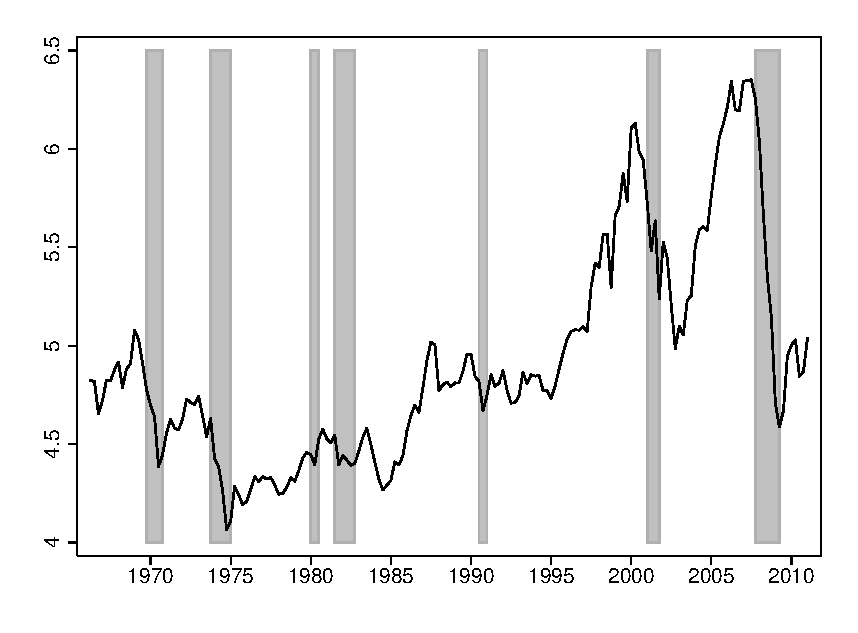
\includegraphics[width=0.49\textheight]{\econtexRoot/Figures/fwyRat}}
		\caption{Net Worth--Disposable Income Ratio}	\label{fwyRat}	
	\end{subfigure}
	\begin{subfigure}[t]{0.49\textheight}
		\centering
		{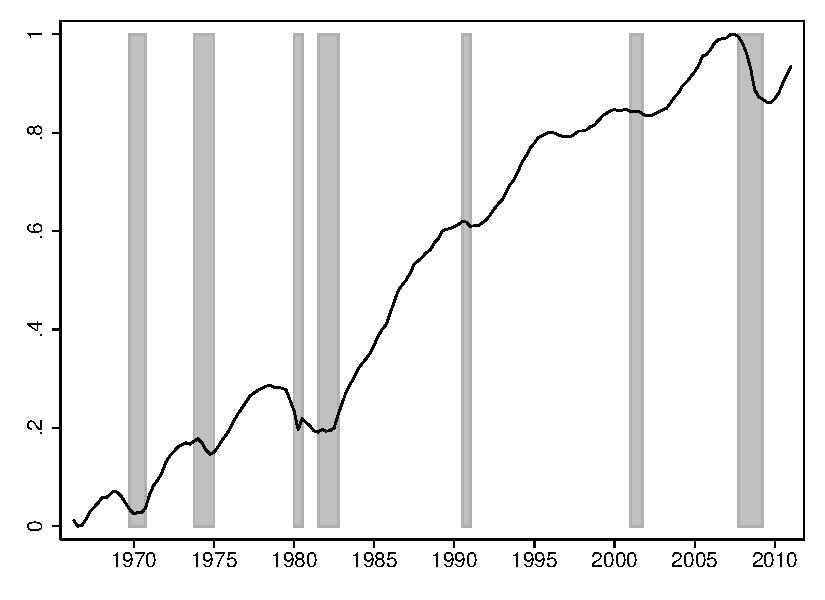
\includegraphics[width=0.49\textheight]{\econtexRoot/Figures/fCEA}}
		\caption{The Credit Easing Accumulated (CEA) Index}\label{fCEA}
	\end{subfigure} \\
	\begin{subfigure}[t]{0.49\textheight}
		\centering
		{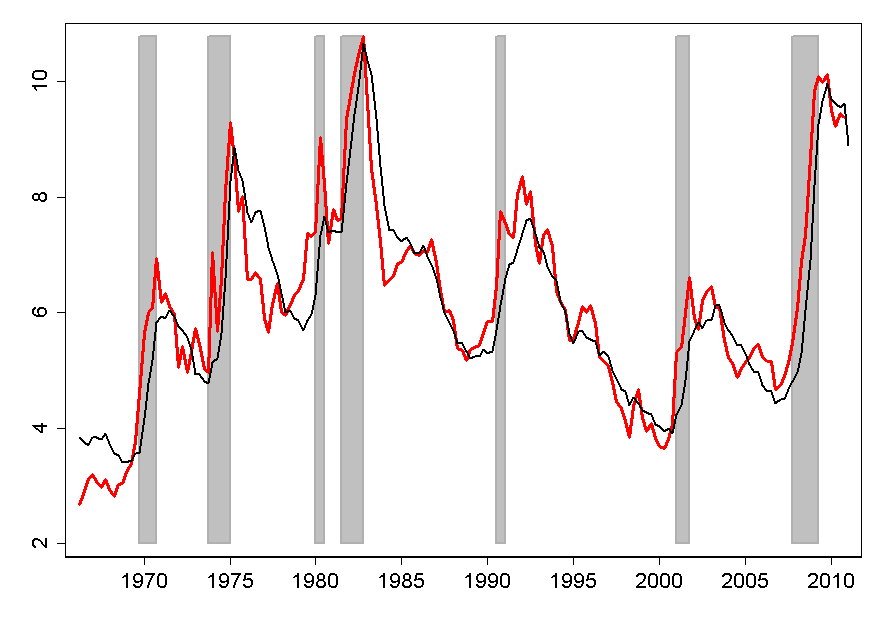
\includegraphics[width=0.49\textheight]{\econtexRoot/Figures/mhoUnem}}
		\caption{Unemployment Risk $\Ex_t u_{t+4}$ and Unemployment Rate}\label{fMho}
	\end{subfigure}
\end{sidewaysfigure}

Our measure of credit availability, which we call the `Credit Easing Accumulated' index ($\CEA$; Figure~\ref{fCEA}) is adapted from work by John Muellbauer and various coauthors (\cite{mue07}, \cite{ducaEtAl10_creditArch} and \cite{admmmCredit}; for a related approach, see \cite{hall:slump}).  It is constructed using a question from the Federal Reserve's Senior Loan Officer Opinion Survey (SLOOS) on Bank Lending Practices. The question asks about banks' willingness to make consumer installment loans now as opposed to three months ago. To calculate a proxy for the \emph{level} of credit conditions, the scores from the survey were accumulated, weighting the responses by the contemporaneous debt-to-income ratio to account for the increasing trend in that variable, and normalizing the result to range between 0 and 1 to make the interpretation of regression coefficients straightforward.  We use the question on installment loans because it is available since 1966; other measures of credit availability, such as for mortgage lending, move closely with the index on consumer installment loans over the sample period when both are available until 2008.  While the two indices diverge in the Great Recession and afterward, this corresponds to the period when there was a massive shift of mortgage origination from banks (the respondents to the SLOOS) to government sponsored entities (Fannie Mae, Freddie Mac, and others).  That shift brings into question the continued relevance of the direct SLOOS index of mortgage lending conditions.  There was no similar profound institutional change in the market for installment lending, which is one reason it might reasonably be interpreted as a consistent indicator of the overall credit environment (given its high correlation with other credit supply indices in the period before the Great Recession).

The CEA index is taken to measure the availability/supply of credit to a typical household as it is affected by factors other than the level of interest rates---for example, through constraints on loan-to-value or loan-to-income ratios, availability of mortgage equity withdrawal and mortgage refinancing. The broad trends in the \CEA\ index seem to reflect well the key developments of the US financial market institutions, which we summarize as follows: Until financial deregulation began in the late 1970s, consumer lending markets were heavily regulated and segmented. After the phaseout of interest rate controls beginning in the early 1980s, the markets became more competitive, spurring financial innovations that led to greater access to credit. Technological progress leading to new financial instruments and better credit screening methods (\cite{pjInfo}), a greater role of nonbanking financial institutions, and the increased use of securitization all contributed to the dramatic rise in credit availability from the early 1980s until the onset of the Great Recession in 2007, at which point a subtantial drop in the \CEA\ index was associated with the funding difficulties and de-leveraging of financial institutions.\footnote{As a caveat, it is important to acknowledge that \CEA\ might to some degree be influenced by developments from the demand rather than the supply side of the credit market.  But whatever its flaws in this regard, indexes of this sort seem to be gaining increasing acceptance as the best available measures of credit supply (as distinguished from credit demand).\\
  The \CEA\ index correlates strongly with measures financial reforms of \cite{abiadEtAl_FinReforms}, and measures of banking deregulation of \cite{demyanykEtAl_JoF07_deregulation} (see panel~A of their Figure~1, p.\ 2786 and Appendix~1).   }

We measure a proxy $\Ex_t u_{t+4}$ for unemployment risk $\mho_t$ using re-scaled answers to the question about the expected change in unemployment in the Thomson Reuters/University of Michigan Surveys of Consumers. %
 In particular, we estimate $\Ex_t u_{t+4}$ using fitted values $\Delta_4 \hat{u}_{t+4}$ from the regression of the four-quarter-ahead change in unemployment rate $\Delta_4 u_{t+4}\equiv u_{t+4}-u_t$ on the answer in the survey, summarized with the balance statistic $\Uexp^{BS}_t$:
\begin{eqnarray*}
\Delta_4 u_{t+4} &=& \alpha_0+\alpha_1\Uexp^{BS}_t+\varepsilon_{t+4},\\
\Ex_t u_{t+4}&=&u_t+ \Delta_4 \hat{u}_{t+4}.
\end{eqnarray*}
The coefficient $\alpha_{1}$ is highly statistically significant, indicating that households do have substantial information about the direction of future changes in the unemployment rate.  As expected, our $\Ex_{t} u_{t+4}$ series is strongly correlated with unemployment rate and predicts its dynamics (Figure~\ref{fMho}).%

\hypertarget{Why-to-2011}{}
\begin{verbatimwrite}{./Highlighted/Why-to-2011.tex}
Data for our empirical measure of credit conditions are available starting 1966q2, and the data we use in estimation cover that date to 2011q4.

We do not use data after 2011 for several reasons. First, personal saving rate statistics are subject to large revisions until some five years  after the first data release (after the BEA receives much higher quality personal income data from the IRS).  To quote \cite{nsSavingRevisions}: ``[M]uch of the initial variation in the personal saving rate across time was meaningless noise.''\footnote{In addition, there were substantial gyrations in the saving rate in 2012 due to a tax-related anomaly (in late 2012 income was boosted by accelerated and special dividend payments and by accelerated bonus payments in anticipation of changes in individual income tax rates in 2013).} As  their paper documents, it is not uncommon for the saving rate to be revised by 3--5 percent of disposable income after several benchmark revisions.


Second, our index of credit availability is increasingly questionable after 2011 because of the apparent divergence in credit conditions for installment and mortgage loans: Various sources (including the Mortgage Credit Availability Index of the Mortgage Bankers' Association; see also \cite{bhutta_mortgageDebt}) document continued tight credit conditions after 2011.  If, as this work suggests, mortgage credit remained tighter than indicated by our installment loans index after 2012, that could explain part of the continued high saving rate in the post-2012 period, which would be mispredicted by a mismeasured credit conditions index.  Alternatively, saving attitudes may have changed after the Great Recession due to the substantial shock of the Great Recession, perhaps because of ``scarring'' effects  (see, e.g., \cite{malmendierSheng}, \cite{jstLeveragedBubbles}, \cite{hallQuantifying}); for evidence that financial crises have much longer-lasting effects than usual business cycle fluctuations, see \cite{rrAftermath}.  All of these are reasons to worry about data from the post-Great-Recession period.
\end{verbatimwrite}
Data for our empirical measure of credit conditions are available starting 1966q2, and the data we use in estimation cover that date to 2011q4.

We do not use data after 2011 for several reasons. First, personal saving rate statistics are subject to large revisions until some five years  after the first data release (after the BEA receives much higher quality personal income data from the IRS).  To quote \cite{nsSavingRevisions}: ``[M]uch of the initial variation in the personal saving rate across time was meaningless noise.''\footnote{In addition, there were substantial gyrations in the saving rate in 2012 due to a tax-related anomaly (in late 2012 income was boosted by accelerated and special dividend payments and by accelerated bonus payments in anticipation of changes in individual income tax rates in 2013).} As  their paper documents, it is not uncommon for the saving rate to be revised by 3--5 percent of disposable income after several benchmark revisions.

Second, our index of credit availability is increasingly questionable after 2011 because of the apparent divergence in credit conditions for installment and mortgage loans: Various sources (including the Mortgage Credit Availability Index of the Mortgage Bankers' Association; see also \cite{bhutta_mortgageDebt}) document continued tight credit conditions after 2011.  If, as this work suggests, mortgage credit remained tighter than indicated by our installment loans index after 2012, that could explain part of the continued high saving rate in the post-2012 period, which would be mispredicted by a mismeasured credit conditions index.  Alternatively, saving attitudes may have changed after the Great Recession due to the substantial shock of the Great Recession, perhaps because of ``scarring'' effects  (see, e.g., \cite{malmendierSheng}, \cite{jstLeveragedBubbles}, \cite{hallQuantifying}); for evidence that financial crises have much longer-lasting effects than usual business cycle fluctuations, see \cite{rrAftermath}.  All of these are reasons to worry about data from the post-Great-Recession period.


\section{Structural Estimation} \label{sStructuralEstimation}

This section estimates the structural model of section~\ref{ssTractableBS} by minimizing the distance between the saving rate implied by the model and its empirical counterpart. %The nonlinear least squares (NLLS) procedure employed here has some advantages over the reduced-form regressions. Besides arguably being more immune to endogeneity and suitable for estimating structural parameters (such as the discount factor), it imposes on the data a structure that makes the parameter values easier to interpret. As Figure~\ref{fig:PhaseDiag} documents, the structural model also explicitly justifies and disciplines non-linearities, which can be important especially during turbulent times, when the shocks are large enough to move the system far from its steady state.

\hypertarget{Estimation-Procedure}{}
\subsection{Estimation Procedure}

In more detail, the structural estimation proceeds as follows. We assume that households observe exogenous movements in unemployment risk $\mho$ and credit availability $\underline{h}$,\footnote{We assume that consumers consider the shocks to $\mho$ and $\underline{h}$ to be permanent.  This assumption is necessary for us to be able to use our tractable model.  While indefensible as a literal proposition (presumably nobody believes the unemployment rate will remain forever where it is today), the high serial correlation of these variables means that the assumption may not be too objectionable.} and that there are simple mappings from our credit availability index $\CEA_{t}$ to the location of the consumers' borrowing constraint $\underline{h}_{t}$ and from measured unemployment expectations $\Ex_{t}u_{t+4}$ to $\mho_{t}$:\footnote{We have also considered a model in which the CEA equation contains an intercept, $\underline{h}(\CEA_{t}) = \bar{\theta}_h+\theta_\CEA \CEA_{t}$. In such model $\bar{\theta}_h$ is estimated to be insignificant and close to 0.  Because that model is close to multi-colinear, we are excluding the intercept from the CEA equation. }
\begin{eqnarray}
 \underline{h}_{t} = \underline{h}(\CEA_{t}) & = & \theta_\CEA \CEA_{t}, \nonumber \\
\mho_{t}= \mho(\Ex_{t}u_{t+4}) & = & \bar{\theta}_\mho+\theta_u \Ex_{t}u_{t+4}. \label{unempEq}
\end{eqnarray}

Collecting the parameters $\Theta=\{\DiscFac,\theta_\CEA,\bar{\theta}_\mho,\theta_u\}$, and the time-$t$ observable variables as $z_{t} = \{\mRat_{t},\CEA_{t},\Ex_{t}u_{t+4}\}$, the model implies a ``saving rate function'' $\sFunc(z_{t};\Theta)$ which we aim to compare to the saving rates observed in the data, $s_t^{\text{meas}}$. Our objective is therefore to find the parameter vector $\hat{\Theta}$ that minimizes the distance between actual saving rates and those implied by the model:
\begin{equation}
  \hat{\Theta}=\argmin \frac{1}{T}\sum_{t=1}^T\big(s_{t}^{\text{meas}}-\sFunc(z_{t}; \Theta)\big)^2. \label{minDist}
\end{equation}

Minimization of \eqref{minDist} is a non-linear least squares problem for which the standard asymptotic results apply. The estimates have the asymptotic normal distribution:
$$
T^{1/2}(\hat{\Theta}-\Theta)\rightarrow_d \mathscr{N}\Big(0, \sigma^2\times\big(\lim_{T\rightarrow\infty} \Ex (\textbf{F}'\textbf{F}/T)\big)^{-1}\Big),
$$
where the variance matrix can consistently be estimated with
$$
\hat\sigma^2\times\big( \hat{\textbf{F}}'\hat{\textbf{F}}\big/ T \big)^{-1}
$$
for $\hat\sigma^2=\frac{1}{T}\sum_{t=1}^T\big(s_{t}^{\text{meas}}-\sFunc(z_{t}; \hat{\Theta})\big)^2$ and the $T\times4$ gradient matrix of the saving rate function $\hat{\textbf{F}}=\nabla_{\Theta'}\sFunc(z_{t}; \hat{\Theta})$ evaluated at $\hat{\Theta}$ (which is calculated numerically).%

\subsection{Estimates and the Model Fit}

Table~\ref{tStructEst} presents the estimation results. The calibrated parameters --- the quarterly real interest rate $\rfree=0.04/4$, quarterly wage growth $\Delta\Wage=0.01/4$ and the coefficient of relative risk aversion $\CRRA=2$ --- take on standard values and meet (together with the estimated discount factor $\DiscFac$) the conditions sufficient for the problem to have a well-defined solution (see \cite{ctDiscrete}).

The estimated quarterly discount factor $\DiscFac=1-0.0065=0.9935$, or $0.974$ at an annual frequency, lies in the standard range.  As for the horizontal shift in the consumption function $\underline{h}_t$ driven by credit availability, the estimates of the scaling factor ${\theta}_\CEA$ implies that $\underline{h}_t$ varies between $0$ and $8.89/4\approx 2.2$, implying that financial deregulation resulted at its peak in an availability of credit in 2007 that was greater than credit availability at the beginning of our sample in 1966 by an amount equal to about 220 percent of annual income (for an average household)---not an unreasonable figure given the rule of thumb that homebuyers can afford a house costing between two and three times their annual income.  %

The estimated intensity of perceived unemployment risk reflects that fact that the risk in our setup is purely permanent: the estimated risk $\mho_t$ ranges between $1.25\times10^{-4}$ and $1.5\times10^{-4}$ per quarter. The peak magnitude of $\mho_t$ (of $1.5\times10^{-4}$) implies that over the life cycle of 50 years or 200 quarters, the workers face a probability of roughly 3 percent to become (permanently) unemployed. Given the average aggregate unemployment rate of roughly 6 percent in our sample and given that much of this risk is in reality transitory, the estimated scaling of $\mho_t$ seems broadly plausible.


The quantitative interpretation of the coefficients in the model is not straightforward, but can be summarized by calculating  that a 30 percent increase in uncertainty (not out of line for a recession) results in a roughly 3 percentage point increase in the saving rate.  A way to judge the plausibility of this prediction is to consider a 30 percent increase in uncertainty in a microeconomically richer model; we have done so using the model of \cite{cstwMPC}, and have found that that model predicts a similar increase in the saving rate as a consequence of a 30 percent increase in its most important measure of uncertainty (the variance of permanent shocks).

\begin{figure}	\caption{The Structural Estimation: Main Results} 
	\centering
	\begin{subfigure}[t]{0.49\textheight}
		\centering
    \addtocounter{figure}{-1}
		{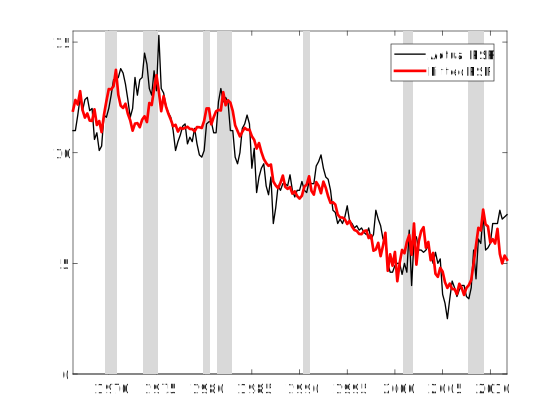
\includegraphics[width=0.475\textheight]{./Figures/fPSR_StructFit}}
		\caption{Actual and Fitted Saving Rate}		\label{fPSR_StructFit}
	\end{subfigure}
	\begin{subfigure}[t]{0.49\textheight}
		\centering
		{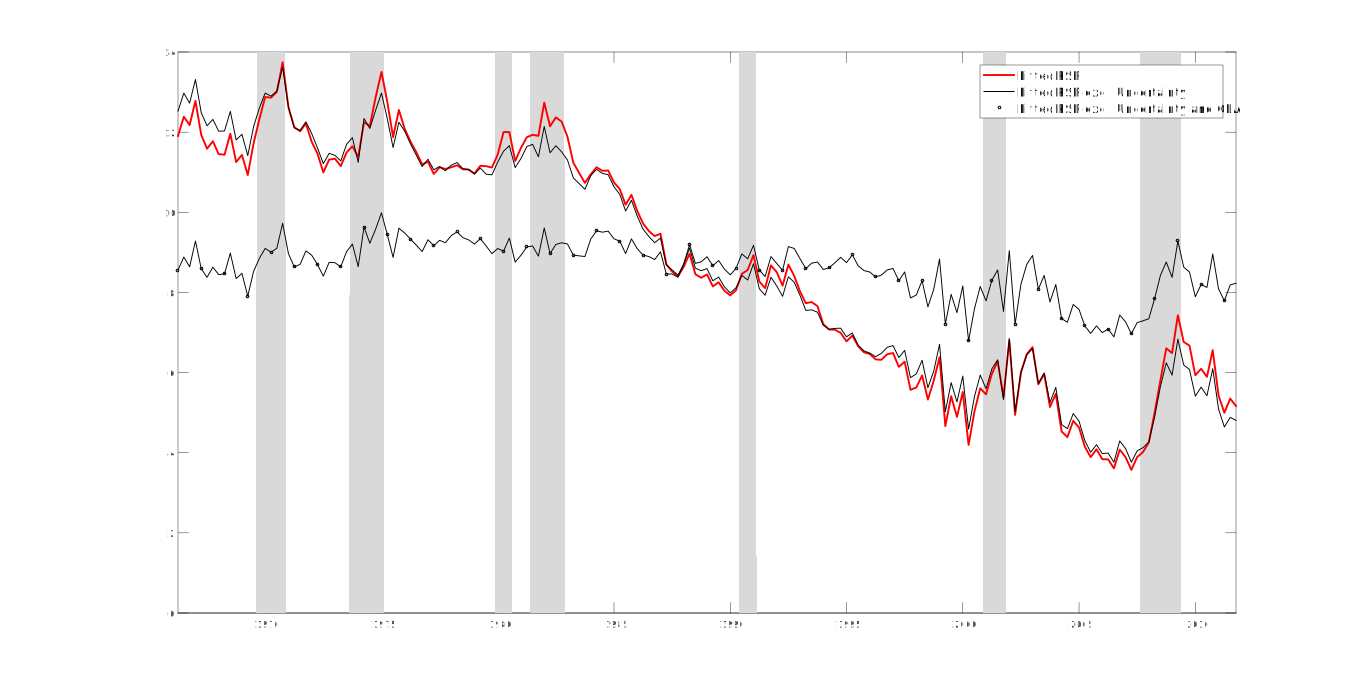
\includegraphics[width=0.475\textheight]{./Figures/fPSR_StructDecomp}}
		\caption{Decomposition of Fitted Saving Rate}\label{fPSR_StructDecomp}
	\end{subfigure}
\end{figure}


\subsection{What Drives the Saving Rate? A Decomposition}

Time-variation in the fitted saving rate arises as a result of movements in its three time-varying determinants: uncertainty, wealth, and credit conditions; Figure~\ref{fPSR_StructDecomp}. To gauge the relative importance of the three variables, we sequentially switch off the channels by setting the series equal to their sample means. For example, the difference between the fitted series  (red/grey line) and the fitted series excluding uncertainty (black line) should be interpreted as the effect of \emph{time variation} in unemployment risk $\mho$ rather than the \emph{total amount} of saving attributable to uncertainty.

The main takeaway from these figures is that the CEA is essential in capturing the trend decline in the PSR between the 1980s and the early 2000s. The wealth fluctuations contribute to a good fit of the model at the business-cycle frequencies, and the cyclical fluctuations in uncertainty magnify the increases in the PSR during recessions.

\hypertarget{The-MPC}{}

The model (black circled line in Figure~\ref{fPSR_StructDecomp}) ascribes roughly 3 percentage points of the increase in the saving rate during the Great Recession to the drop in net worth, which amounted to roughly 200~percent of disposable income (Figure~\ref{fwyRat}), implying a marginal propensity consume out of wealth of $3/200=0.015$. This value is on the low end of the range produced by existing representative agent models, though models that incorporate habit formation can generate MPC's well below 1 percent.

Our model does not incorporate transitory shocks to income, but because market resources $\mRat$ are wealth plus income, the model could be interpreted as suggesting an MPC out of transitory income that would be near the same low number as the MPC out of wealth, very far from the micro estimates, which \cite{cstwMPC} characterize as usually falling between 0.2 and 0.7.

We believe that heterogeneity is essential to explain this discrepancy.  In a model like that of \cite{cstwMPC}, wealth shocks mostly hit wealthy people -- who have low MPC's; and income shocks (like stimulus checks) hit the whole population, which includes many low-wealth people who have high MPC's.  If this is the right explanation, an RA model (ours included) is by its fundamental nature incapable of reconciling the conflict. In addition, a substantial proportion of shocks to net worth are driven by housing wealth, for which evidence suggests that the MPC is likely lower than for liquid assets (including increases from income tax rebates; for a compelling quasi-natural experiment on the size of housing wealth effects, see \cite{ktvHousingWealthEffect}).

Combining all three channels, the model implies an increase in the saving rate of about 5 percentage points between 2007 and 2010  (red line in Figure~\ref{fPSR_StructDecomp})---not far from the actual change.  Our model's comparatively low MPC out of wealth but substantial roles for the other two channels suggests that much of what has been interpreted as pure ``wealth effects'' in the prior literature may actually have reflected precautionary or credit availability effects that are correlated with wealth (a finding in line with much of the household-level evidence, including \cite{hurstStafford}, \cite{cooper_housingCollateral}, \cite{asWealthEffect}  and others, who stress the role of credit availability and collateral constraints).


\hypertarget{sReducedFormRegressions}{}

\section{Empirical Evaluation of Alternative Models} \label{sReducedFormRegressions}

Here we argue that our model has advantages over the chief alternatives that can be readily evaluated.

\hypertarget{Quadratic-Utility}{}

\subsection{Quadratic Utility} \label{sec:Quadratic}

Since \cite{hallRandomWalk}, an optimizing model with quadratic utility has been an influential benchmark to model aggregate consumption dynamics (both literally and, effectively, in linearized DSGE models). The key distinction from our theoretical model in section~\ref{ssTractableBS} is that, in contrast to CRRA utility, under quadratic utility uncertainty has no effect on consumption dynamics; quadratic-utility households do not engage in precautionary saving and do not have a wealth target (other than the current level of wealth).

The model without uncertainty turns out to be distinctly inferior to our buffer stock saving model.  We have already seen above in Table~\ref{tStructEst} that the intercept $\bar{\theta}_\mho$ and the sensitivity to uncertainty $\theta_u$ enter very significantly the  unemployment risk equation \eqref{unempEq} of the structural model.  This evidence is confirmed in a reduced form linear regression estimation, where business-cycle variation in labor market uncertainty is strongly related to the PSR, both on its own and controlling for other variables (columns~1 and~3 of Table~\ref{tRFall}, respectively). The results imply that a~1~percentage point increase in expected unemployment rate increases the saving rate by roughly 0.2--0.6 percentage points.\footnote{We have also considered other measures of uncertainty, such as financial market or economic policy uncertainty (\cite{bbdUncertainty}), but our measure of labor market uncertainty, which is much more closely tied to a rigorous theory, also turns out to work better as a determinant of personal saving.}

These results confirm a large body of complementary evidence on how uncertainty affects aggregate consumption and saving going back to 1990s). Recently, the evidence based on household-level data has shown that uncertainty is also important for macroeconomic outcomes (\cite{bfjstUncertain}, \cite{kv_microMacro} and many others). These findings, mostly based on `normal' (shallow) recessions,  were further strengthened during the Great Recession when (according to \cite{kmpHandbook} and the references in footnote~\ref{foot_housingLit}) uncertainty amplified the drop in house prices, employment and consumption.


\hypertarget{Demographics-and-Saving}{}
\subsection{Demographics and Saving} \label{DemSav}

\hypertarget{fig:AddDataSeries}{}
\begin{sidewaysfigure}		\caption{Additional Data Series: Demographics, Government Saving and Inequality} \label{fig:addVars}
	\centering
	\begin{subfigure}[t]{0.49\textheight}
	%\addtocounter{figure}{-1}	
    \centering
		{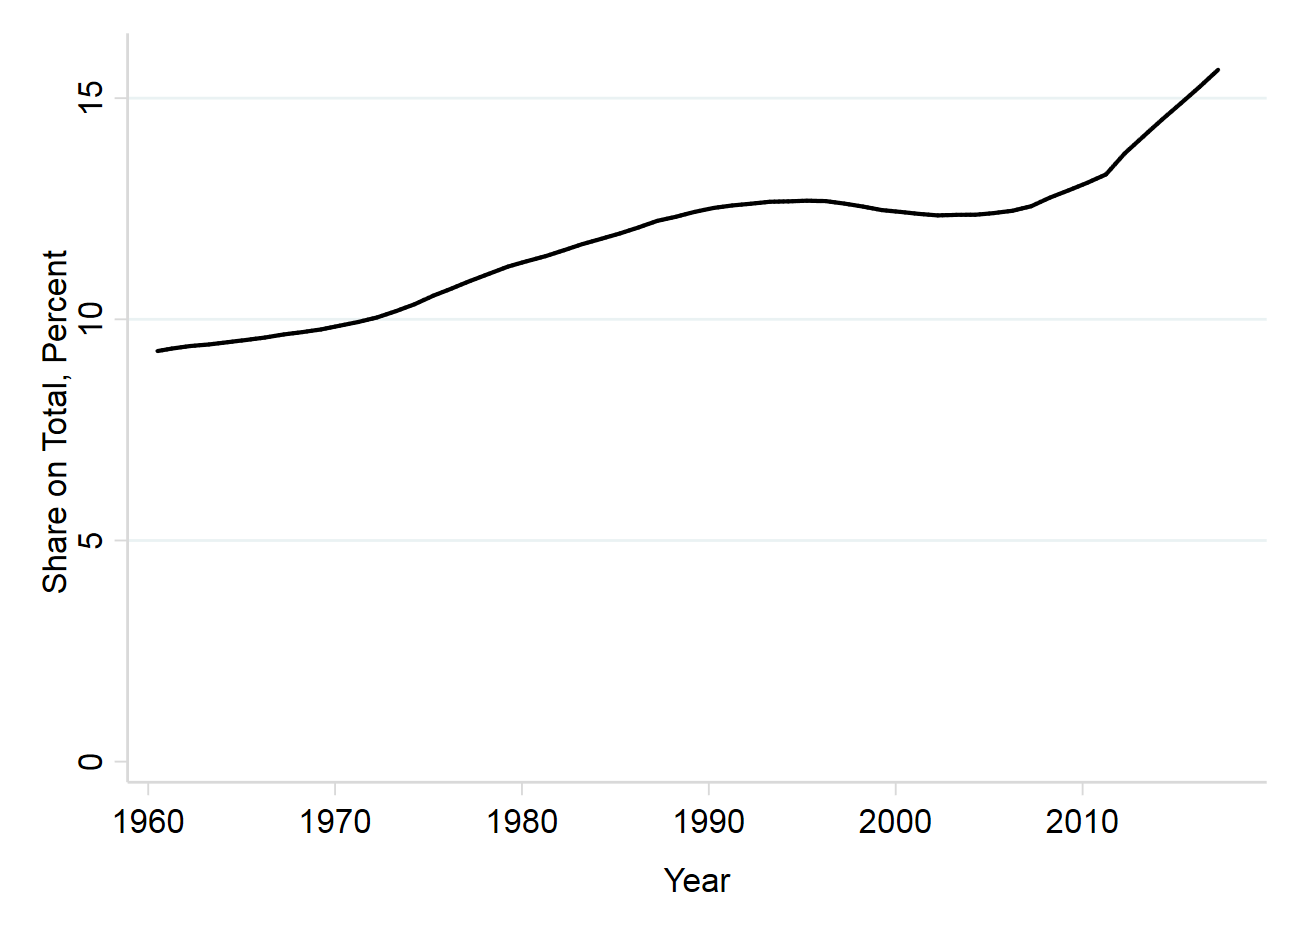
\includegraphics[width=0.475\textheight]{\econtexRoot/Figures/sharePop65plus}}
		\caption{Share of Population Above 65 Years (Old-Age Dependency Ratio)}		\label{f65+}
	\end{subfigure}
	\begin{subfigure}[t]{0.49\textheight}
		\centering
		{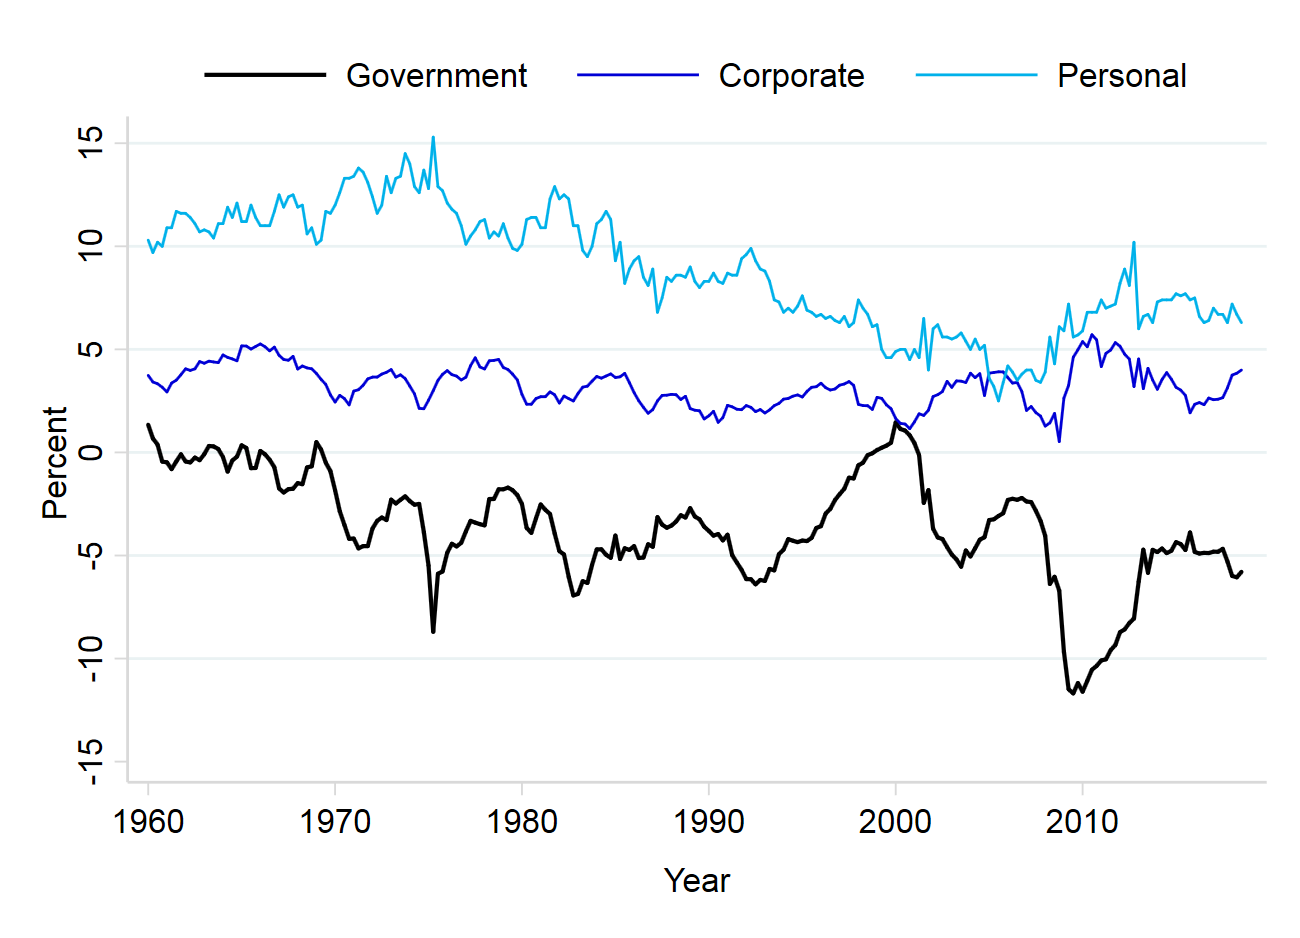
\includegraphics[width=0.475\textheight]{\econtexRoot/Figures/govSavingShare}}
		\caption{Government and Corporate Saving (as Fraction of GDP)} \label{fgovSav}
	\end{subfigure} \\
	\begin{subfigure}[t]{0.49\textheight}
		\centering
		{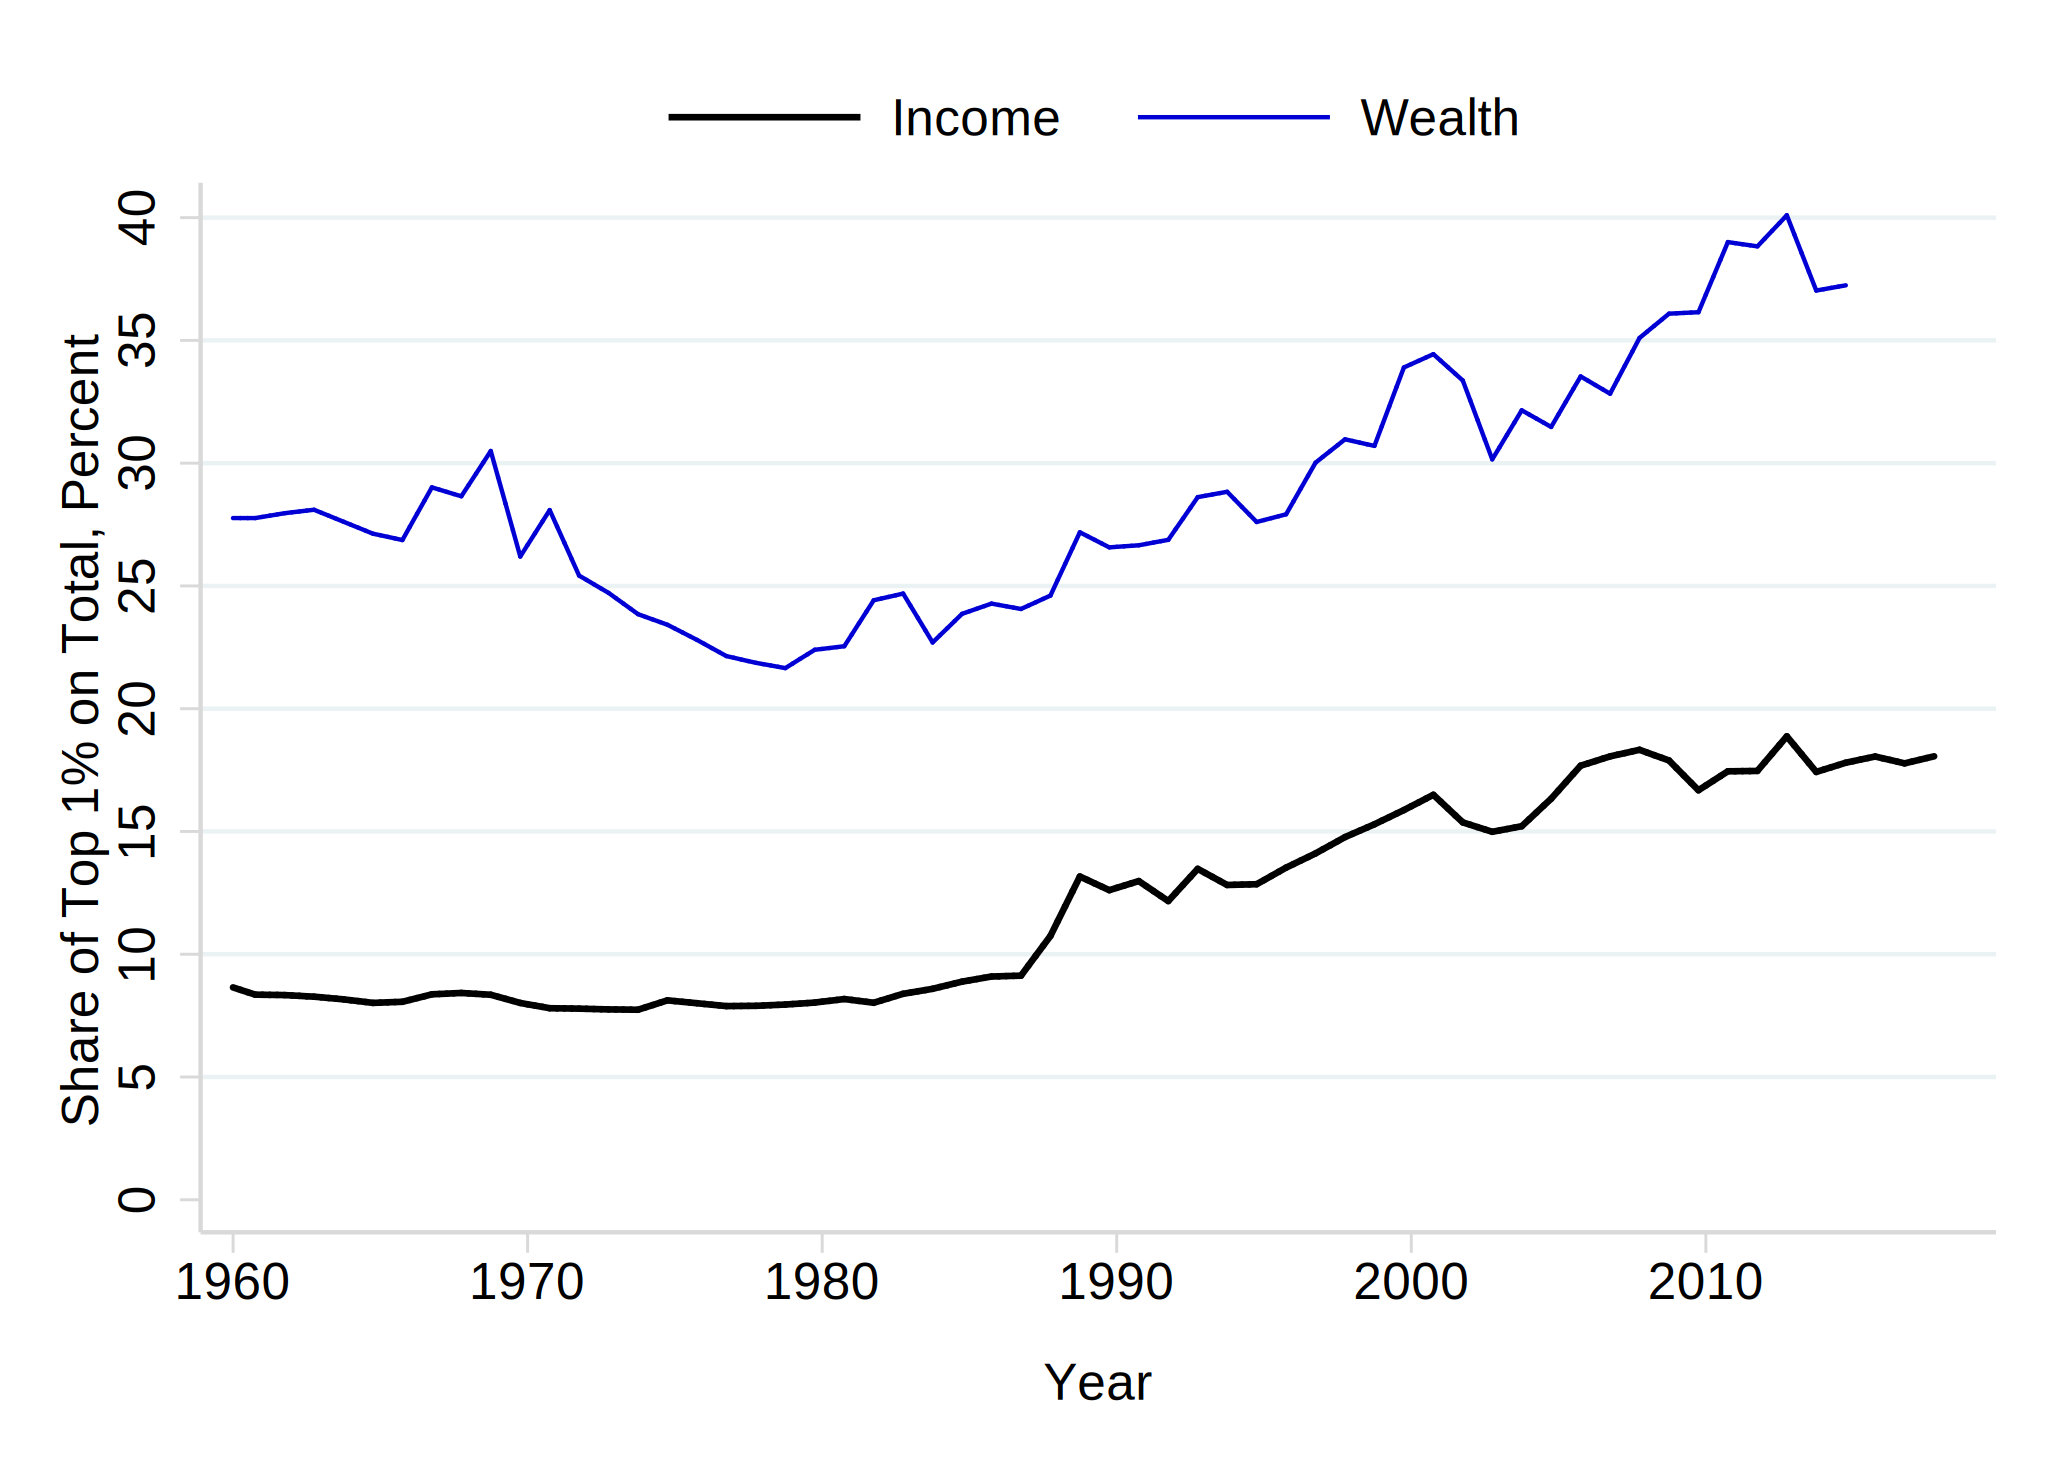
\includegraphics[width=0.475\textheight]{\econtexRoot/Figures/topIncomeShare}}
		\caption{Share of Top 1 Percent, Income and Wealth} \label{fTopShare}
	\end{subfigure}
\end{sidewaysfigure}



A long tradition of work, stemming from the seminal work of \cite{mb54}, examines the implications of demographic change for saving using calibrations and simulations of various life-cycle models (usually in an OLG setup). 
Overall, this strand of work has concluded that at the higher frequencies (e.g., annual) demographic changes do not substantially affect changes in saving because they are both small and very slow-moving (\cite{scWhySavSoLow}, \citet{parker_nberma_spendthrift} and many others).

If demographic trends could provide a compelling explanation for the long-term decline in the saving rate leading up to 2007, that might constitute a plausible alternative to our story based on increased credit availability in the era of financial deregulation.  But \cite{auerbachKotlikoffDemographicsAndSaving} and related papers argued persuasively in the early 1990s that the first-order implication of demographics was that there should be a sustained \textit{rise} in the saving rate for many years until the baby boom generation hit its peak earnings years around 2000--2005, and a declining saving rate thereafter.  This is precisely the opposite of the actual pattern (the baby boom generation began exiting the ``high-saving'' phase of life and entering the supposedly ``low-saving'' retirement phase during exactly the interval when the saving rate stopped declining and then rose).

\hypertarget{Kotlikoff}{}
This point is roughly captured in Figure~\ref{f65+} which plots the old-age dependency ratio, which began rising faster around 2010 when large numbers of baby boomers began reaching retirement age.
In Table~\ref{tRFall}, column~2 we estimate that the coefficient on the old-age dependency ratio is negative, which would suggest that the increase in the share of people older than 65~years should have \emph{reduced} the saving rate, so the correlations go the wrong way for a demographic story (confirming the large prior literature after \cite{auerbachKotlikoffDemographicsAndSaving} that failed to find meaningful demographic effects).\footnote{For China a separate strand of work (e.g., \cite{curtisEtAl} and \cite{imrohroglu_China}) uses a newer generation of these models to investigate the implications of demographic change.  This work typically argues that demographic change did substantially contribute to the massive increase in saving (from around 5 percent in the 1970s to more than 25 percent in the 2010s).  On the other hand, the importance of population aging in cross-country studies of household saving (for example, \cite{bloomEtAl_JME07} and \cite{bosworthChodorowReich07}) appears to be largely driven by the experience of Japan and Korea---countries well ahead of the United States in the population aging process.
}

\hypertarget{Reduced-Form-vs-Structural-Models-of-Saving}{}

\subsection{Reduced-Form vs Structural Models of Saving}

We now ask to what extent the main features of the structural model of section~\ref{ssTractableBS} can be summarized in a simple reduced-form linear regression:
\begin{equation}
s_t=\gamma_1+\gamma_m m_t +\gamma_{\CEA}\CEA_t+\gamma_{Eu}\Ex_t u_{t+4}+\varepsilon_t. \label{srOLS}
\end{equation}
This specification can be readily estimated using OLS estimators (Table~\ref{tRFall}, column~3) and, at a minimum, can be interpreted as summarizing basic
stylized facts about the data.

We have mentioned (in section~\ref{sec:Quadratic}) that the estimates of the ``Baseline'' model \eqref{srOLS} are significant and explain more than 90 percent of variation in the saving rate. As expected from the structural model, the point estimates indicate a strong negative correlation of saving with net wealth and credit conditions, and a positive correlation with unemployment risk.

The coefficient on the Credit Easing Accumulated index is highly statistically significant with a $t$-statistic of more than 14. (Of course, this $t$-statistic should be taken with a several grains of salt given the obvious trends in both variables, and the cautionary literature about regressions of trends on trends; but aside from demographics (which go the wrong way), there are no other variables that are core constituents of standard saving models that have had powerful trends like this, so the case for spurious correlation is weaker than it sometimes is).  The point estimate of $\gamma _{\CEA}$ implies that increased access to credit over the sample period until the Great Recession reduced the PSR by about 8 percentage points of disposable income. In the aftermath of the Recession, the \CEA\ index declined between 2007 and 2010 by roughly $0.11$
 as credit supply tightened, contributing roughly $0.64$
 percentage point to the increase in the saving rate.  Finally, once the three variables are included jointly, the time trend ceases to be significant (column~4).

Given how well the baseline linear reduced-form model captures the saving rate, one might wonder what value is added by construction of the structural model we proposed earlier.  A first point to make here is that when we simulate the estimated version of our model and perform linear regressions on the corresponding generated data, the result is very close to being linear (the $R^{2}$ is 0.974).  Essentially, therefore, the difference between the two approaches is that the OLS regression puts no restrictions at all on the linear relationships between the variables, while the structural estimation puts stringent requirements that those linear relationships be tightly constrained to the small subset of nearly linear relationships that is a good approximation to the structural theory.  The fact that the $R^{2}$ from the structural estimation is essentially the same as for the unrestricted model (both of them round to $0.91$) was by no means inevitable and indicates that the structure imposed by the model does no violence to the data.%\footnote{The Mincer--Zarnowitz horse race between the models puts weight of 0.72 on the structural model.}

\hypertarget{Why-Estimate-a-Structural-Model}{}

\subsubsection{Why Estimate a Structural Model When OLS Works Fine?}

Because structural estimation restricts empirical relationships to those that are compatible with a theory, structural models by their intrinsic nature fit the data worse than an unrestricted data-fitting exercise; the advantages of structural modeling (articulated below) can nevertheless make such estimation worth the sacrifice in data-fitting ability.  In the case at hand, however, the structural model fits the data nearly as well as an unrestricted OLS regression.  Thus, in our context, the case for structural modeling is stronger than in the usual case where there is a significant penalty in data-fitting ability.

Some of the advantages of having a structural model are:
\begin{itemize}
\item If the structure imposed is one that has considerable backing from other contexts or kinds of data, it is less likely that the fit of the model to the data is spurious (in the sense of failing to capture any reliable or causal economic relationship).
\item The structural model can provide insights that could not be obtained from the reduced form model.  For example, the ``overshooting'' result implied by the structural model might have important consequences for business cycle dynamics even if the fit of the structure that embodies those dynamics is statistically inferior to the reduced form fit.
  \item The structural model has implications for ways to test the ideas using data other than those on which it was estimated.  In this case, for example, the structural model would suggest that it would be useful to look at regional or local data in which the endogeneity of aggregate asset prices and credit conditions could be controlled for by looking at differences in unemployment expectations and saving responses across regions in an aggregate economy where most of the movements in the other explanatory variables are not region-specific.
  \end{itemize}

\subsection{Further Robustness Checks}

Columns 5 and 6 of Table~\ref{tRFall} summarize the correlations of the personal saving rate with two variables that some theories suggest might be related to it: government saving (Figure~\ref{fgovSav}) and income inequality (Figure~\ref{fTopShare}).

Column~5 reports that there is indeed a negative correlation between government and personal saving, though the size of the coefficient, $-0.15$, implies only a modest crowding out. More than a support for the Ricardian equivalence---the hypothesis that households observing higher government saving should save less themselves (as they should expect lower taxes in the future)---the finding seems to reflect reverse causality between private and public saving, the fact that during recessions government saving falls (e.g., due to higher outlays on unemployment insurance), while personal saving rises for precautionary reasons (see work of \cite{elmendorfMankiw} and many others).


Finally,  in column~6 we evaluate whether  growing income inequality (shown in Figure~\ref{fTopShare})
 has resulted in an increase in the aggregate saving rate: Microeconomic evidence
 points to high personal saving rates among the higher-permanent-income households
 (\cite{carroll:richsave}; \cite{dszRichSave}), whose share on total income has been rising.  Having experimented with numerous measures of the top shares of \cite{Piketty_Saez2003}, we find little evidence of a substantial and statistically significant correlation between saving and income inequality.

\begin{comment}

 However, the econometric evidence is mixed.
 We have experimented with numerous income inequality series of \cite{Piketty_Saez2003} (updated through 2010)
 in our regressions: we included income shares of the top 10, 5, 1, 0.5, and 0.1 percent of the income distribution,
 either with or without capital gains. None of these 10 series were statistically significant in the full 1960--2010
 sample; one of the estimated specifications is reported in Table~\ref{tOLS}. Some of the inequality measures
 were statistically significant in a shorter, 1980--2010, sample. In this specific sub-sample (results not reported here),
 the coefficients on credit conditions and net wealth remained highly statistically significant, although the coefficient
 on credit conditions tended to be more negative than in the baseline specification. The coefficient on unemployment expectations
 became insignificant, which is also natural since income inequality fluctuates over the business cycle.



\jbemph{Possibly mention  [Rising Inequality, Ricardian Equivalence, \dots? ]}\\
Mention also the irrelevance of the Ricardian equivalence? ie recently all saving went up, household, corporate and government.

Ricardian equivalence: Households observing higher government saving should save less themselves (as they should expect lower taxes in the future)

We have known at least since \citet{parker_nberma_spendthrift}'s section~2 REq doesn't matter (for personal saving).  And nothing has changed since then; possibly add a chart with gov saving as fraction of GDP.
\end{comment}



\section{Conclusions} \label{conclusions}

We show that a simple representative-consumer model of buffer stock saving can match most of the time-series variation in the aggregate US personal saving rate over the past 50 years. In the model, saving depends on the gap between the `target' and actual wealth, with the target determined by credit availability and uncertainty.

We estimate that these three factors---credit availability, shocks to household wealth, and movements in income uncertainty proxied by unemployment risk---have all been important in driving the saving rate. In particular, the relentless expansion of credit supply between the early-1980s and 2007 (likely largely reflecting financial innovation and liberalization), along with higher asset values and consequent increases in net wealth (possibly also partly attributable to the credit boom) encouraged households to save less out of their disposable income. At the same time, the fluctuations in wealth and labor income uncertainty, for instance during and after the burst of the information technology and credit bubbles of 2001 and 2007, can explain the bulk of business cycle fluctuations in personal saving.

The model we estimate could be extended to analyze the implications of the `overshooting' of saving in response to business-cycle shocks. For example, the model suggests that in a recession an optimizing government might want to counteract the part of the consumption decline that reflects overshooting. In an economy rendered non-Ricardian by liquidity constraints and/or uncertainty, the existence of precautionary saving thus provides a potential rationale for counter-cyclical fiscal policy.

More generally, the simple buffer stock saving model we estimate could provide insights into the current debate about the role household heterogeneity for macroeconomic outcomes.  The model is both easy to solve and provides a setup to meaningfully analyze the effects on uncertainty on the macro-economy.  Consequently, the model could be a useful middle ground between a setup with a realistic but complex description of household heterogeneity (HANK) and a simple two-agent spender--saver setup (TANK) that cannot accommodate roles for credit availability or uncertainty.

\small

\clearpage\pagebreak
\bibliography{economics,\econtexRoot/cssUSSaving,\econtexRoot/cssUSSaving-Add}


\begin{table}
 \caption{ Calibration and Structural Estimates} \label{tStructEst}
 \begin{center}
 \begin{tabular}{@{}lld{6}@{}}
 \multicolumn{3}{c}{ $s_t^{\text{theor}}=s_t^{\text{theor}}\big(\Theta; \mRat_t-\check{\mRat}(\bar{h}_t,\mho_t)\big)$, } \\
 \multicolumn{3}{c}{ $\bar{h}_t=\bar{\theta}_\h+\theta_{\CEA} \CEA_t$, } \\
 \multicolumn{3}{c}{  $\mho_t=\bar{\theta}_\mho+\theta_u \Ex_tu_{t+4}$. } \\
 \toprule
  \multicolumn{1}{l}{Parameter} & \multicolumn{1}{l}{Description} & \multicolumn{1}{c}{Value}  \\
 \midrule
   \multicolumn{3}{l}{Calibrated Parameters} \\
   $\rfree$ & Interest Rate & \multicolumn{1}{c}{0.04/4} \\
  $\Delta \Wage$ & Wage Growth & \multicolumn{1}{c}{0.01/4} \\
  $\CRRA$  & Relative Risk Aversion & 2 \\
 \midrule
  \multicolumn{3}{l}{Estimated Parameters $\Theta=\{\Discount, \bar{\theta}_h,\theta_{\CEA},\bar{\theta}_\mho,\theta_u\}$}\\
  $\Discount$ & Discount Rate & 1- 0.0064^{***}  \\
  & & (0.0016 ) \\
  $\bar{\theta}_h$ & Scaling of $\CEA_t$ to $\bar{h}_t$ & 0.8751^{}  \\
  & & (1.6636 ) \\
  ${\theta}_{\CEA}$ & Scaling of $\CEA_t$ to $\bar{h}_t$ & 5.2504^{**}  \\
  & & (2.6012 ) \\
  $\bar{\theta}_\mho$ & Scaling of $\Ex_tu_{t+4}$ to $\mho_t$ & 6.3218 \times{10^{-5}}^{**}  \\
  & & (3.1300\times{10^{-5}} ) \\
  ${\theta}_u$ & Scaling of $\Ex_tu_{t+4}$ to $\mho_t$ & 2.6079 \times{10^{-4}}^{}  \\
  & & (4.7670 \times{10^{-4}} ) \\
 \midrule
  $\bar{R}^2$ & &  0.884  \\
  DW stat & &  1.057  \\
 \midrule
   & Sample average of $\CEA_t$  & 0.5129  \\
   & Sample average of $\Ex_tu_{t+4}$  & 0.0618  \\
  \bottomrule
 \end{tabular}
 \end{center}
  {\footnotesize Notes: Quarterly calibration. Estimation sample: 1966q2--2011q1. $\{{}^*,{}^{**},{}^{***}\}={}$Statistical significance at $\{10,5,1\}$ percent.  Standard errors (in parentheses) were calculated with the delta method.  Parameter estimates imply sample averages of   3.57 and 0.000079 for $\bar{h}_t$ and $\mho_t$, respectively. } \\  
\end{table}



\begin{table}
\caption{ Reduced-Form Regressions} \label{tRFall} \small
\begin{center}
\begin{tabular}{@{}ld{6}d{6}d{6}d{6}d{6}d{6}@{}}
\multicolumn{7}{c}{ $s_t=\gamma_0+\gamma_m m_t+\gamma_{\CEA}\CEA_t+ \gamma_{Eu}\Ex_t u_{t+4}+\gamma'X_t+\varepsilon_t$ } \\
\toprule
   & & & \multicolumn{2}{c}{Reduced-Form} & \multicolumn{2}{c}{Additional Variables} \\
  \cmidrule(l){4-5} \cmidrule(l){6-7}
  Model & \multicolumn{1}{c}{Uncertainty} & \multicolumn{1}{c}{Demographics} & \multicolumn{1}{c}{Baseline} & \multicolumn{1}{c}{Time Trend}& \multicolumn{1}{c}{Gov Sav} & \multicolumn{1}{c}{Ineq} \\
\midrule
$\gamma_0$ & 11.750^{ ***}  & 29.504^{ ***}  & 17.157^{ ***}  & 15.535^{ ***}  & 17.588^{ ***}  & 18.553^{ ***}\\
 & (0.462)  &  (5.257)  &  (1.589)  &  (2.004)  &  (1.589)  & (1.804)\\
$\gamma_m$   & &-1.596^{ ***}  & -0.894^{ ***}  & -0.618^{ *}  & -0.862^{ ***}  & -1.321^{ ***}\\
 & & (0.362)  &  (0.261)  &  (0.341)  &  (0.269)  & (0.410)\\
 $\gamma_{\CEA}$   & & -4.444^{ ***}  & -7.909^{ ***}  &-4.156^{ **}  & -8.149^{ ***}  & -9.545^{ ***}\\
 & & (1.451)  &  (0.556)  &  (2.098)  &  (0.565)  & (1.249)\\
$\gamma_{Eu}$  & 0.551^{ ***}  & 0.264^{ ***}  & 0.202^{ ***}  & 0.347^{ ***}  & 0.028^{ }  & 0.181^{ ***}\\
 & (0.059) & (0.068)  &  (0.064)  &  (0.105)  &  (0.074)  & (0.065)\\
 $\gamma_{t}$   & -0.055^{ ***}  & & &-0.025^{ }  & & \\
 &(0.002) & & & (0.015)  &    &  \\
 $\gamma_\text{old}$   &  & -0.861^{ **} & & & &   \\
 &    &  (0.365) & & &  &   \\
 $\gamma_\text{gov sav}$     & & & & &-0.152^{ **}  &  \\
 &      & & & &(0.063) &  \\
 $\gamma_\text{inc share}$   &  & & & & &0.190^{ }\\
 & &   & & & &(0.144)  \\
\midrule
 $\bar{R}^2$  & 0.910  &  0.918  & 0.911  &  0.914  &  0.916  & 0.913\\
 F stat p val  & 0.000 & 0.000  &  0.000  &  0.000 & 0.000 & 0.000\\
DW stat  & 0.761  & 0.848  & 0.732  &  0.769  & 0.682  & 0.771\\
\bottomrule
\end{tabular}
\end{center}
\showEstTime{Estimated: 13 Mar 2019, 18:27:56}
 {\footnotesize Notes: Estimation sample: 1966q2--2011q4. $\{{}^*,{}^{**},{}^{***}\}={}$Statistical significance at $\{10,5,1\}$ percent. Newey--West standard errors, 4 lags.}
\end{table}


\clearpage



\clearpage{\Large\textbf{
Supplemental Materials---Not for Publication
}}
\clearpage
\appendix



%----------------------------------------------------------------------------------------
% Appendix 3 shows the derivation of incorporating severance into ctDiscrete framework. -- 1/30/2013
% It should be put right after the subsection:
% \subsection*{Stochastic Properties of Disposable Income and Saving for a Rainy Day}

\section*{Appendix 3: Extension of Derivation of Target Wealth to Include Unemployment Insurance}

The model described in \cite{ctDiscrete} assumes that income for
unemployed/retired households is zero.  A step in the direction of
realism is to recognize the existence (in most countries) of an unemployment
insurance system that guarantees some level of income to unemployed
persons.  The implications of such a system are straightforward to
model if we assume that the unemployment insurance benefit is a
constant proportion of the labor income earned in the first year of unemployment if not losing job.

In the perfect foresight context, receiving a constant payment with
perfect certainty is equivalent to receiving a lump sum ``severance''
payment whose value is equal to the PDV of the stream of future UI
payments.  Thus, for simplicity, we assume
$\SeverancePayment=\SeveranceRatio\cdot\labor\Wage$, which means
individuals will receive one-period severance payment $\SeverancePayment$ in the amount of
a certain ratio $\SeveranceRatio$ to labor income of the period when they first lose their jobs. After that, they will not receive any unemployment
insurance benefit.

The only modifications of the decision problem are to add
the severance payment and a corresponding lump-sum tax into the
dynamic budget constraint (DBC) of employed consumers in
\cite{ctDiscrete},
\begin{displaymath}
    \mLev_{t+1}=\left\{
    \begin{array}{ll}
    \bLev_{t+1}+\labor_{t+1}\Wage_{t+1}-\TaxUI_{t+1} & \mbox{w.p. } \urate\\
    \bLev_{t+1}+\SeverancePayment_{t+1} & \mbox{w.p. }1-\urate,
    \end{array}
    \right.
\end{displaymath}
where $\mLev$, $\bLev$ and $\labor\Wage$ denote market resources,
assets and labor income respectively. We let $\TaxUI=\urate\times
\SeverancePayment$ to ensure a balanced budget for the unemployment
insurance system.\footnote{Each period, proportion
  $\urate$ of employed consumers lose their jobs, i.e., the ``exit
  rate'' in the current labor market is $\urate$.  In order to raise a
  corresponding amount of revenues, we need to assume that there is a
  ``birth rate'' of $\urate$ of new employed consumers, which means a
  same proportion of consumers are entering the labor market each
  period. Combined with the assumption that $\TaxUI=\urate\times
  \SeverancePayment$, the severance payment and the severance payment are
  balanced.}

Following \cite{ctDiscrete}, we have the following condition derived from the Euler equation,
\begin{equation}
  1  = \PGro^{-\CRRA}\Rfree\Discount \left\{(1-\urate)\left(\frac{\cRatE_{t+1}}{\cRatE_{t}}\right)^{-\CRRA}+\urate \left(\frac{\cU_{t+1}}{\cRatE_{t}}\right)^{-\CRRA}\right\},
\end{equation}
where nonbold variables represent the bold variables normalized by
labor income $\labor\Wage$. Superscripts $e$ and $u$ represent the two
possible states.

To find the $\Delta c^e=0$ and $\Delta m^e=0$ loci, we let
$c_{t+1}^e=c_t^e\equiv c^e$ and $m_{t+1}^e=m_{t}^e\equiv m^e$. Given
$c_{t+1}^u=m_{t+1}^u\kappa^u$ ($\kappa^u$ is the MPC of an unemployed
consumer), combined with the modified DBC above, we have
\begin{equation*}
1 = \PGro^{-\CRRA}\Rfree\Discount \left\{(1-\urate)+\urate \left(\frac{\MPCU(\Rnorm(m^e-c^e)+\SeveranceRatio)}{\cRatE}\right)^{-\CRRA}\right\}.
\end{equation*}

Rearranging terms, the $\Delta c^e=0$ locus can be characterized as
\begin{equation}
\overbrace{\left(\frac{\PGro^{\CRRA}(\Rfree\Discount)^{-1}-\erate}{\urate}\right)^{1/\CRRA}}^{\straight}=\left(\frac{c^e}{(\Rnorm(m^e-c^e)+\SeveranceRatio)\MPCU}\right).
\end{equation}

Given the modified DBC of employed consumers, the $\Delta m^e=0$ locus becomes
\begin{equation}
m^e=\Rnorm(m^e-c^e)+(1-\urate\SeveranceRatio).
\end{equation}

Given the two equations above, we are able to obtain the exact formula for target wealth $\check{m}$, which is the steady state value of $m^e$. Following \cite{ctDiscrete}, define $\eta \equiv \Rnorm \MPCU \straight$. We have
\begin{eqnarray}
\frac{\eta\check{m}+\frac{\eta\SeveranceRatio}{\Rnorm}}{\eta+1}&=&(1-\Rnorm^{-1})\check{m}+\frac{1-\urate\SeveranceRatio}{\Rnorm}=\check{c}\nonumber\\
\left(\frac{1}{\Rnorm}-\frac{1}{\eta+1}\right)\check{m} &=& \frac{1}{\Rnorm}\left(1-\urate\SeveranceRatio-\frac{\eta\SeveranceRatio}{\eta+1}\right)\nonumber\\
\check{m}&=& \frac{(\eta+1)(1-\urate\SeveranceRatio)-\eta\SeveranceRatio}{\eta+1-\Rnorm}.
\end{eqnarray}

Clearly, target wealth decreases when the severance payment becomes more generous and it can even be negative if we make the severance ratio $\SeveranceRatio$ large enough.
%-----------------------------------------------------------------------------------------


\section{Comparison of Alternative Measures of Credit Availability}


\hypertarget{fCreditAvailability}{}
\begin{figure}
\caption{Alternative Measures of Credit Availability \label{fCreditAvailability}}
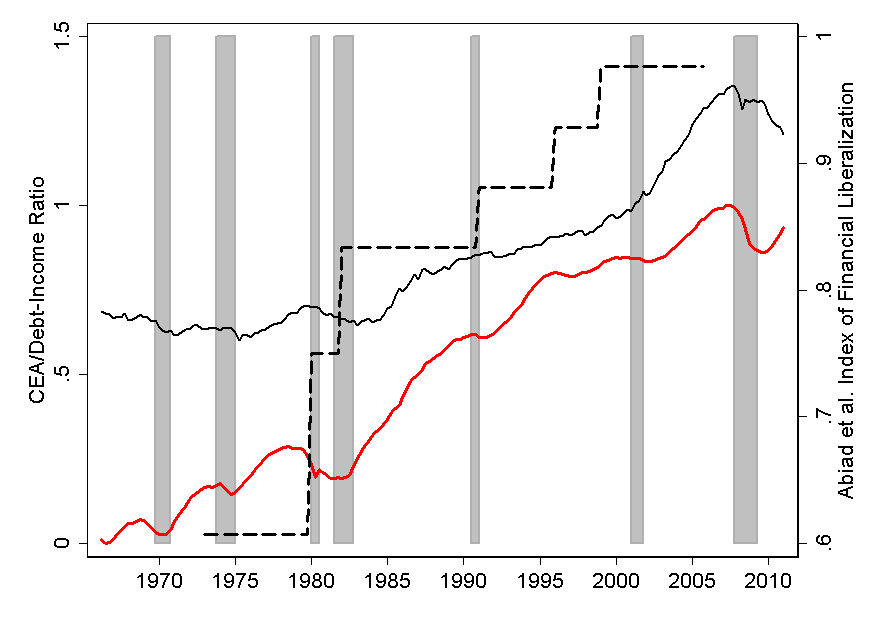
\includegraphics{\econtexRoot/Figures/fCreditAvailability_compare}

\footnotesize
Legend: Debt--disposable income ratio: Thin black line, CEA index: Thick red/grey line, the \cite{abiadEtAl_FinReforms} Index of Financial Liberalization: Dashed black line. Shading---NBER recessions.\\[0mm]
\tiny Sources: Federal Reserve, accumulated scores from the question on change in the banks' willingness to provide consumer installment loans from the Senior Loan Officer Opinion Survey on Bank Lending Practices, \url{http://www.federalreserve.gov/boarddocs/snloansurvey/}; \cite{abiadEtAl_FinReforms}; Flow of Funds, Board of Governors of the Federal Reserve System.
\end{figure}

Figure~\ref{fCreditAvailability} compares three measures of credit availability: our baseline CEA index, the Index of Financial Liberalization constructed by \cite{abiadEtAl_FinReforms} for a number of countries including the United States, and the ratio of household liabilities to disposable income.

The \citeauthor{abiadEtAl_FinReforms} index is a mixture of indicators of financial development: credit controls and reserve requirements, aggregate credit ceilings, interest rate liberalization, banking sector entry, capital account transactions, development of securities markets and banking sector supervision. The correlation coefficient between this measure and CEA is about 90 percent.

For comparison, the figure also includes the ratio of liabilities to disposable income (from the Flow of Funds), which is however determined influenced by the interaction between credit supply and demand.

\clearpage

\section{Reduced Form Regressions with Saving Rate Generated by the Structural Model}

  
\begin{table}
\caption{ Reduced-Form Regressions with Saving Rate Estimated by the Structural Model} \label{tRFall_model} \small
\begin{center}
\begin{tabular}{@{}ld{6}d{6}d{6}d{6}d{6}d{6}@{}}
\multicolumn{7}{c}{ $s_t=\gamma_0+\gamma_m m_t+\gamma_{\CEA}\CEA_t+ \gamma_{Eu}\Ex_t u_{t+4}+\gamma'X_t+\varepsilon_t$ } \\
\toprule
   & & & \multicolumn{2}{c}{Reduced-Form} & \multicolumn{2}{c}{Additional Variables} \\
  \cmidrule(l){4-5} \cmidrule(l){6-7}
  Model & \multicolumn{1}{c}{Uncertainty} & \multicolumn{1}{c}{Demographics} & \multicolumn{1}{c}{Baseline} & \multicolumn{1}{c}{Time Trend}& \multicolumn{1}{c}{Gov Sav} & \multicolumn{1}{c}{Ineq} \\
\midrule 
$\gamma_0$ & 11.689^{ ***}  & 18.994^{ ***}  & 16.254^{ ***}  & 16.093^{ ***}  & 16.215^{ ***}  & 16.330^{ ***}\\
 & (0.182)  &  (1.126)  &  (0.636)  &  (0.710)  &  (0.633)  & (0.646)\\
$\gamma_m$   & &-0.912^{ ***}  & -0.756^{ ***}  & -0.729^{ ***}  & -0.759^{ ***}  & -0.780^{ ***}\\
 & & (0.110)  &  (0.099)  &  (0.113)  &  (0.099)  & (0.117)\\
 $\gamma_{\CEA}$   & & -7.316^{ ***}  & -8.085^{ ***}  &-7.713^{ ***}  & -8.064^{ ***}  & -8.174^{ ***}\\
 & & (0.292)  &  (0.112)  &  (0.621)  &  (0.114)  & (0.309)\\
$\gamma_{Eu}$  & 0.555^{ ***}  & 0.237^{ ***}  & 0.223^{ ***}  & 0.238^{ ***}  & 0.239^{ ***}  & 0.222^{ ***}\\
 & (0.025) & (0.018)  &  (0.017)  &  (0.030)  &  (0.021)  & (0.016)\\
 $\gamma_{t}$   & -0.055^{ ***}  & & &-0.002^{ }  & & \\
 &(0.001) & & & (0.004)  &    &  \\
 $\gamma_\text{old}$   &  & -0.191^{ ***} & & & &   \\
 &    &  (0.071) & & &  &   \\
 $\gamma_\text{gov sav}$     & & & & &0.014^{ }  &  \\
 &      & & & &(0.014) &  \\
 $\gamma_\text{inc share}$   &  & & & & &0.010^{ }\\
 & &   & & & &(0.033)  \\
\midrule 
 $\bar{R}^2$  & 0.975  &  0.989  & 0.988  &  0.988  &  0.988  & 0.988\\
 F stat p val  & 0.000 & 0.000  &  0.000  &  0.000 & 0.000 & 0.000\\
DW stat  & 1.167  & 2.331  & 2.213  &  2.219  & 2.237  & 2.217\\
\bottomrule
\end{tabular}
\end{center}
\showEstTime{Estimated: 25 Apr 2019, 15:54:05}
 {\footnotesize Notes: Estimation sample: 1966q2--2011q4. $\{{}^*,{}^{**},{}^{***}\}={}$Statistical significance at $\{10,5,1\}$ percent. Newey--West standard errors, 4 lags.}
\end{table}











\clearpage
\jbemph{Additional Pieces of Text---To Be Deleted (Eventually)}

\hypertarget{fOLS-fit-time-compare}{}
\begin{figure}
\caption{The Fit of the Baseline Model and the Time Trend---Actual and Fitted PSR (Percent of Disposable Income)}
\label{fOLS_fit_time_compare}
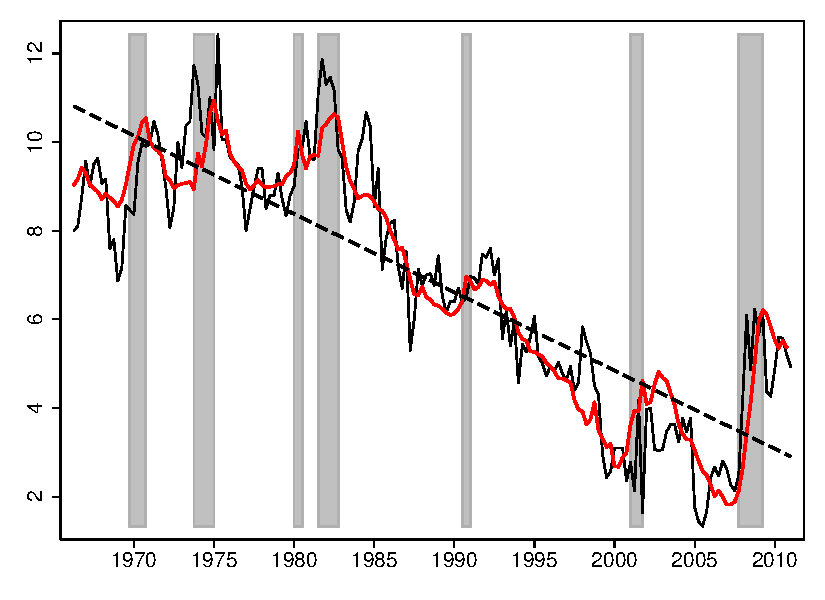
\includegraphics{\econtexRoot/Figures/fOLS_fit_time_compare}

\footnotesize
Legend: Actual PSR: Thin black line, Baseline model: Thick red/grey line, Time trend: Dashed black line. Shading---NBER recessions.\\[0mm]
\tiny Sources: Bureau of Economic Analysis, authors' calculations.
\end{figure}



Table~\ref{tOLS} presents a second battery of specification checks of
the baseline model shown again for reference as the first `model.'  The second model (Uncertainty) investigates the effects of adding to the baseline regression an
alternative proxy for uncertainty: the
\cite{bfjstUncertain} index of macroeconomic and
financial uncertainty.%
\footnote{See \cite{baker_policyUncertainty} for related work measuring \emph{economic policy} uncertainty.
}
 The new variable is statistically insignificant
and the coefficients on the previously included variables are broadly
unchanged, suggesting that our baseline uncertainty measure is more
appropriate for our purposes (which makes sense, as personal saving is
conducted by persons, whose uncertainty is likely better captured by
our measure of labor income uncertainty than by the
\cite{bfjstUncertain} measure of firm-level shocks).

The third model (Lagged $s_{t-1}$) explores the implications of adding lagged saving to the list of regressors.  Often in empirical
macroeconomics, the addition of the lagged dependent variable is unjustified by the underlying theory, but nevertheless is required
for the model to fit the data.  Here, however, serial correlation in saving is a direct implication of the model (below we will show that the degree of serial correlation implied by the model matches the empirical estimate fairly well).  The implication arises because deviations of actual wealth from target wealth ought to be long-lasting if the saving rate cannot quickly move actual wealth to the target.  As expected, the coefficient is highly statistically significant.  However, this positive autocorrelation only captures near-term stickiness and has little effect on the long-run dynamics of saving. Indeed, the coefficients from the baseline roughly equal their long-term counterparts from the model with lagged saving rates (that is, coefficient estimates pre-multiplied by $2.5$, or $1/(1-\gamma_s)=1/(1-0.60)$).\footnote{Note that with the inclusion
  of lagged saving, the Durbin--Watson statistic becomes close to 2,
  suggesting that whatever serial correlation exists in the
  other specifications reflect simple first order autocorrelation of
  the errors.}

The fourth model (Debt) explores the role of the debt--income ratio. The variable could be relevant for two reasons. First, it could partly account for the fact that debt is held by a different group of people than assets and consequently net worth might be an insufficient proxy for wealth. Second, debt might also reflect credit conditions (although---as mentioned above---we prefer the CEA index because in principle it isolates the role of credit supply from demand). The regression can thus also be interpreted as a horse-race between the CEA and the debt--income ratio. In any case, while the coefficient $\gamma_d$ has the correct (negative) sign, it is statistically insignificant and its inclusion does not substantially affect estimates obtained under the baseline specification.


\hypertarget{fFullControls}{}
\begin{figure}
\caption{The Fit of the Baseline Model and the Model with Full Controls (of Table~\ref{tOLS})---Actual and Fitted PSR (Percent of Disposable Income)}
\label{fFullControls}
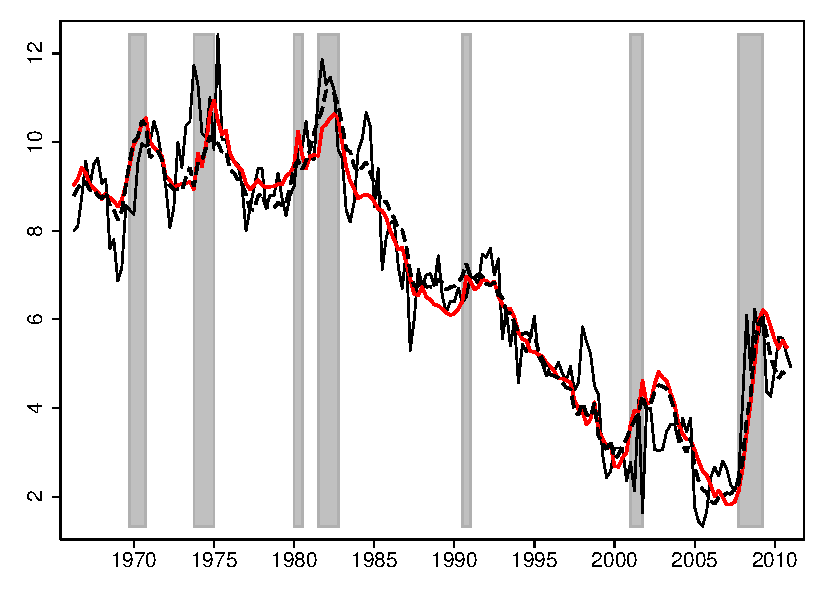
\includegraphics{\econtexRoot/Figures/fFullControls}

\footnotesize
Legend: Actual PSR: Thin black line, Baseline model: Thick red/grey line, Model with full control variables: Dashed black line. Shading---NBER recessions.\\[0mm]
\tiny Sources: Bureau of Economic Analysis, authors' calculations.
\end{figure}

The seventh model (DB Pensions) examines whether the shift from defined benefit to defined contribution pension plans
 may also have had a measurable effect on the aggregate saving rate. Aggregate data on the size of defined-benefits pension
 plans are not readily available; the NIPA provides the relevant series only since 1988. As an initial experiment,
 we calculated the share of employer contributions accruing to the defined benefit plans as a percent of total contributions;
 however, this variable was not statistically significant in our regressions (sample 1988--2010). As an alternative, we compiled
 a measure of household saving adjusted for the defined-benefit pension plans from various research publications
 by the Bureau of Economic Analysis (BEA; \cite{kmitchSaving}, \cite{prSaving}) and Congressional Budget Office (CBO; \cite{CBOSaving}). Subsequently, we calculated ``a pension gap,'' defined as the difference between the headline saving rate
 and the BEA/CBO adjusted saving rate, and included this gap variable in our regressions (sample: 1960--2007). The gap is statistically
 significant with a coefficient of about 0.7. This suggests that the shift from defined benefit to defined contribution pension plans
 may have reduced the aggregate saving rate. However, this effect appears small in economic terms: the contribution of the changing pension system
 to the overall decline in the saving rate since the 1980s is only about 1 percentage point of disposable income. The coefficients on the baseline series (credit conditions, net wealth, unemployment expectations) remain highly statistically significant in this regression.

The eighth and ninth models (High Tax Bracket and Low Tax Bracket) provide a first-pass test of the effects of tax policy
 on aggregate saving by including the data on the highest and lowest marginal tax rates in our regressions. Neither of the two
 variables are statistically significant.


Finally, to explore how much endogeneity may matter,%
\footnote{As mentioned above, wealth is lagged by one quarter to alleviate
  endogeneity in OLS regressions.  However, a standard concern about reduced-form regressions like \eqref{srOLS} is that the OLS coefficient estimates might be biased because the regressions do not adequately account for all relevant right-hand size variables (such as expectations about income growth; see also Appendix~2 for further discussion).
  }
  the specification ``IV'' re-estimates
the baseline specification using the IV estimator. Instruments are
the lags of net wealth, unemployment risk and---crucially---the Financial Liberalization Index of \cite{abiadEtAl_FinReforms} (described in Appendix~1).
The FLI is an alternative measure of credit conditions constructed using the records about legal and regulatory changes in the banking sector. The index intends to capture exogenous changes in credit conditions. While it is a rough approximation as it reflects only the most important events (see also Figure~\ref{fCreditAvailability} in Appendix~1), the profile of the FLI matches well that of the CEA. The
estimated coefficients remain broadly unchanged compared with the baseline specification.


\subsection{Sub-Sample Stability}

When the model is estimated only using the post-1980 data in Table~\ref{tOLS_subSample} (Post-1980), its fit measured by the $\bar{R}^2$ actually improves, in contrast with many other economic relationships, 
whose goodness-of-fit deteriorated in the past 20 years.  The F test does not reject the proposition that the regression coefficients have remained stable over the sample period. Allowing for a structural break at the start of the Great Recession in 2007q4 (column `Pre-2008') does not much affect the baseline estimates. (The estimated values of the post-2007 interaction dummies and their standard errors are of course not particularly meaningful because the relevant sub-sample only consists of 13 observations.)

To anticipate the potential criticism that saving rate regressions are difficult to interpret because aggregate income shocks reflect a mix of transitory and persistent factors, we have also re-estimated our regressions with alternative measures of disposable income (see Appendix 2) which exclude a range of identifiable temporary shocks such as fiscal stimulus and extreme weather. There was little econometric evidence that transitory movements in aggregate disposable income are substantial and our econometric results basically did not change.

\subsection{Saving Rate Decompositions}

Table~\ref{tPred} reports an in-sample fit of the baseline model and
the model Interact with the \CEA--uncertainty interaction term of
Table~\ref{tOLSprelim}, together with the contributions of the individual
variables to the explained increase in the saving rate between 2007
and 2010. Two principal conclusions emerge. First, both models
(especially the latter) are able to capture well the observed change
in the saving rate. Second, the key explanatory factors in saving were the changes in wealth and uncertainty, with
credit conditions (as measured by \CEA) playing a less important role.  While the
change in the trajectory of the \CEA\ index is quite striking (see
Figure~\ref{fCEA}), and may explain the sudden academic interest in the
role of household credit over the business cycle (see the papers cited
in the introduction), this evidence suggests that the rise in saving
cannot be primarily attributed to the decline in credit availability.  If
correct, this finding is particularly important at the present
juncture because it suggests that however much the health of the
financial sector continues improving, the saving rate is likely to remain high so
long as uncertainty remains high and household wealth remains impaired
(compared, at least, to its previous heights).





\section{Appendix 2: Stochastic Properties of Aggregate Disposable Income}

\subsection{Measurement of Disposable Income}

\hypertarget{fDispIncG}{}
\begin{figure}
\caption{Growth of Real Disposable Income (Percent) \label{fDispIncG}}
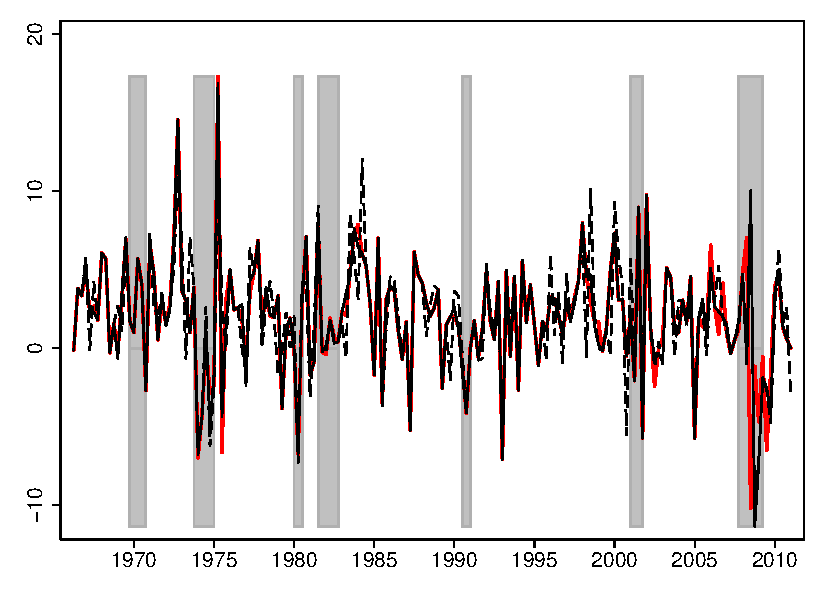
\includegraphics{\econtexRoot/Figures/fDispIncG}

\footnotesize
Legend: BEA disposable income: Thick red/grey line,  ``Less cleaned'' disposable income series: Thin black line, ``More cleaned'' disposable income series: Dashed black line. Shading---NBER recessions.\\[0mm]
\tiny Sources: Bureau of Economic Analysis, authors' calculations.
\end{figure}

\hypertarget{fPSRcompare}{}
\begin{figure}
\caption{Personal Saving Rate (Percent of Disposable Income) \label{fPSRcompare}}
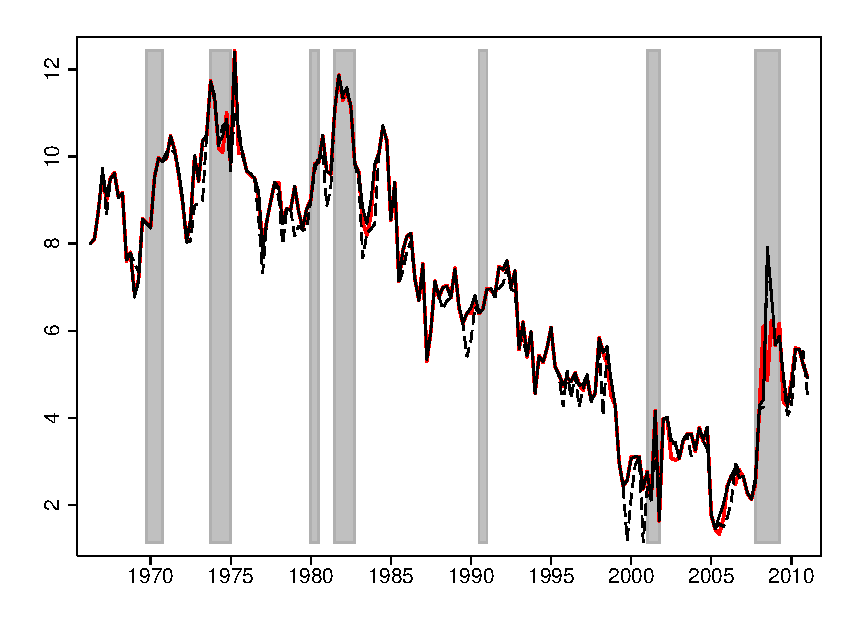
\includegraphics{\econtexRoot/Figures/fPSRcompare}

\footnotesize
Legend: BEA personal saving rate: Thick red/grey line, PSR calculated with the ``less cleaned'' income series: Thin black line, PSR calculated with the ``more cleaned'' income series: Dashed black line. Shading---NBER recessions.\\[0mm]
\tiny Sources: Bureau of Economic Analysis, authors' calculations.
\end{figure}

This appendix investigates the properties of three measures of disposable income: the official series produced by the BEA and two alternative ``cleaned'' series, in which we aim to exclude transitory income shocks due to temporary events, such as weather and fiscal policy. Specifically, we have removed the following events from the official disposable income series using regressions:
\bi
\item The dollar amounts of temporary rebate checks during 1975, 2008, and 2009 fiscal stimulus episodes.
\item Dummies for the 20 costliest tropical cyclones using data from the National Weather Service.
\item Dummies for quarters with unusually high or low cooling degree days, and unusually high or low heating degree days (the dummy has a value of 1 whenever the seasonally-adjusted series are more than 2 standard deviations above or below its mean).
\item Dummies for quarters with unusually high or low national temperature, and unusually high or low precipitation (again, using the 2 standard deviations criterion).
\item Separate dummies for snowstorms or heat waves which were deemed unusually extensive and damaging (these events do not necessarily overlap with the episodes identified from the national temperature and cooling/heating degree days data).
\ei

The ``less cleaned'' disposable income series removes from published data the contributions of stimulus and heating/cooling day extremes. The ``more cleaned'' series removes all the sources of transitory fluctuations outlined above.



\subsection{Stochastic Properties of Disposable Income and Saving for a Rainy Day}

The classic paper by \cite{cam87} derived that the permanent income hypothesis implies that saving is negatively  related to future expected income growth.  This appendix investigates the univariate stochastic properties of disposable income and the relationship between saving and income, or the lack of it, in Tables~\ref{tUnivarYPSR} and \ref{tCampbell87}, respectively.

Table~\ref{tUnivarYPSR} documents that all three disposable income series are statistically indistinguishable from a random walk. This means that (changes in) the series are unpredictable using their own lags. In particular, for the income series in log-level, the first autocorrelations are very close to 1 and the augmented Dickey--Fuller test does not reject the null of a unit root. In contrast, for income \emph{growth}, the first and other autocorrelations are zero, as also documented by the p values of the Box--Ljung Q statistic, and the ADF test (of course) strongly rejects  a unit root.

Table~\ref{tCampbell87} reports the estimates of $\alpha_1$ the sensitivity of the saving rate to future income growth:
\begin{equation}
s_t=\alpha_0+\alpha_1 \Delta y_{t+1}+ \varepsilon_t, \label{cambellRainyDayReg}
\end{equation}
which is motivated by \cite{cam87}, who derives that under the permanent income hypothesis the coefficient $\alpha_1$ is negative, as households save more when they are pessimistic about future income growth.

Overall, the estimates suggest that coefficient $\alpha_1$ is statistically insignificant and small, especially when the full sample, 1966q2--2011q1, is used and when income growth $\Delta y_{t+2}$ enters the regression \eqref{cambellRainyDayReg}, which might be justified because of time aggregation issues. While there is some evidence of a negative coefficient in the pre-1985 sample (which overlaps with the sample 1953q2--1984q4 considered by \cite{cam87}), the relationship seems to break down in the past 20 years.


\newpage

  
\begin{table}
\caption{ Additional Saving Regressions II.---Sub-sample Stability} \label{tOLS_subSample} %\small 
\begin{center}
\begin{tabular}{@{}ld{6}d{6}d{6}@{}}
\multicolumn{4}{c}{ $s_t=\gamma_0+\gamma_m m_t+\gamma_{\CEA}\CEA_t+ \gamma_{Eu}\Ex_t u_{t+4}+\varepsilon_t$ } \\
\toprule
     Model & \multicolumn{1}{c}{Baseline} & \multicolumn{1}{c}{Post-1980}& \multicolumn{1}{c}{Pre-2008}  \\
\midrule 
$\gamma_0$ & 15.226^{ ***}  & 16.692^{ **}  & 16.002^{ ***}\\
 & (2.157)  &  (7.571)  &  (1.340)\\
$\gamma_m$   & -1.183^{ ***}  & -1.503^{ }  & -1.327^{ ***}\\
 & (0.347)  &  (1.248)  &  (0.215) \\
 $\gamma_{\CEA}$   & -6.121^{ ***}  & -4.999^{ **}  & -6.002^{ ***}\\
 & (0.573)  &  (2.000)  &  (0.369 ) \\
$\gamma_{Eu}$  & 0.287^{ ***}  &  0.298^{ **}  &  0.288^{ ***}\\
 &   (0.075)  &   (0.136)  &   (0.053 ) \\
 $\gamma_{\text{0post80}}$/$\gamma_{\text{0post07}}$  &   & -1.479^{ }  &  11.891^{ }\\
 &  &  (7.905)   & (24.356)  \\
 $\gamma_{m\text{post80}}$/$\gamma_{m\text{post07}}$  &   &  0.559^{ }  & -1.234^{ }\\
 & &  (1.289)  & (1.556)  \\
 $\gamma_{\CEA\text{post80}}$/$\gamma_{\CEA\text{post07}}$  &   &  -2.350^{ }  & 5.426^{ }\\
 &  & (2.135)  & (12.414) \\
 $\gamma_{Eu\text{post80}}$/$\gamma_{Eu\text{post07}}$  &   & -0.098^{ }  & -1.027^{ }\\
 &   &  (0.162)  &  (0.715) \\
\midrule 
 $\bar{R}^2$  & 0.895  & 0.899  & 0.903\\
 F stat p val  & 0.00000  & 0.00000  & 0.00000\\
 F p val post-80/pre-08 & & 0.16665  &  0.00012\\
DW stat  & 0.933  & 0.967  & 1.052\\
\bottomrule
\end{tabular}
\end{center}
\showEstTime{Estimated:  1 Sep 2012, 23:49:08}
 {\footnotesize Notes: Estimation sample: 1966q2--2011q1. $\{{}^*,{}^{**},{}^{***}\}={}$Statistical significance at $\{10,5,1\}$ percent. Newey--West standard errors, 4 lags. $\CEA$ is the Credit Easing Accumulated Index. Pre-2008: Heteroscedasticity robust standard errors (because post-2007 sample consists of only 13 observations).}
\end{table} 

\hypertarget{tPred}{}  
\begin{table}
\caption{ Personal Saving Rate---Actual and Explained Change, 2007--2010} \label{tPred} 
\begin{center}
\begin{tabular}{@{}lrrc@{}}\\
\toprule
     Variable & \multicolumn{1}{c}{Baseline }& \multicolumn{1}{c}{Interact }& \multicolumn{1}{c}{Actual $\Delta s_t$ }\\
\midrule 
$\gamma_m\times\Delta m_t$ & $ -1.18 \times -1.39 = 1.64 $ & $ -1.37 \times -1.39 = 1.90 $ & \\
$\gamma_\CEA\times\Delta \CEA_t$ & $ -6.12 \times -0.11 = 0.64 $ & $ -4.60 \times -0.11 = 0.48 $ &  \\
$\gamma_{Eu}\times\Delta \Ex_t u_{t+4} $ & $ 0.29 \times 4.33 = 1.24 $ & $ 0.38 \times 4.33 = 1.67 $ & \\
$\gamma_{uC}\times\Delta (\Ex_t u_{t+4}\times\CEA_t) $ &  & $ -0.32 \times 3.33 = -1.07 $ &  \\\midrule
Explained $\Delta s_t$ &  3.53 &  2.98 & 2.93\\
\bottomrule
\end{tabular}
\end{center}
\end{table} 


  
\begin{table}
\caption{ Preliminary Saving Regressions and the Time Trend} \label{tOLSprelim} \small 
\begin{center}
\begin{tabular}{@{}ld{6}d{6}d{6}d{6}d{6}d{6}d{6}@{}}
\multicolumn{8}{c}{ $s_t=\gamma_0+\gamma_m m_t+\gamma_{\CEA}\CEA_t+ \gamma_{Eu}\Ex_t u_{t+4}+\gamma_t t+\gamma_{uC} (\Ex_t u_{t+4}\times\CEA_t)+\varepsilon_t$ } \\
\toprule
  Model & \multicolumn{1}{c}{Time} & \multicolumn{1}{c}{Wealth} & \multicolumn{1}{c}{CEA} & \multicolumn{1}{c}{Un Risk}& \multicolumn{1}{c}{All 3} & \multicolumn{1}{c}{Baseline} & \multicolumn{1}{c}{Interact} \\
\midrule 
$\gamma_0$ & 11.954^{ ***}  & 25.202^{ ***}  & 9.321^{ ***}  & 8.241^{ ***}  & 14.896^{ ***}  & 15.226^{ ***}  & 15.550^{ ***}\\
 & (0.608)  &  (1.727)  &  (0.574)  &  (0.420)  &  (2.558)  &  (2.157)  & (2.556)\\
$\gamma_m$   & &-2.606^{ ***}  & & & -1.124^{ ***}  & -1.183^{ ***}  & -1.368^{ ***}\\
 & & (0.319)  &  & &   (0.423)  &  (0.347)  &  (0.456) \\
 $\gamma_{\CEA}$   & & & -14.138^{ ***}  & &-5.472^{ ***}  & -6.121^{ ***}  & -4.604^{ ***}\\
 & & & (1.736)  &   &   (1.936)  &  (0.573)  &  (1.721)\\
$\gamma_{Eu}$  & & & & 0.670^{ ***}  & 0.316^{ ***}  & 0.287^{ ***}  & 0.385^{ ***}\\
 &   &   &  & (0.055)  &   (0.117)  &   (0.075)  &   (0.108 ) \\
 $\gamma_{t}$   & -0.044^{ ***}  &  -0.025^{ ***}  &  0.042^{ ***}  &  -0.048^{ ***}  &  -0.005^{ }  & & 0.004^{ }\\
 & (0.005)& (0.003) & (0.011) & (0.002) & ( 0.014 ) & & (0.014)\\
 $\gamma_{uC}$   &  & & & & & & -0.321^{ **}\\
 &   &  &  & & & & (0.158)   \\
\midrule 
 $\bar{R}^2$  & 0.703  & 0.846  & 0.825  & 0.881  & 0.895  & 0.895  & 0.899\\
 F stat p val  & 0.00000  & 0.00000  & 0.00000  & 0.00000  & 0.00000  & 0.00000  & 0.00000\\
DW stat  & 0.305  & 0.686  & 0.500  & 0.863 & 0.936 & 0.933 & 0.980\\
\bottomrule
\end{tabular}
\end{center}
\showEstTime{Estimated:  1 Sep 2012, 23:48:41}
 {\footnotesize Notes: Estimation sample: 1966q2--2011q1. $\{{}^*,{}^{**},{}^{***}\}={}$Statistical significance at $\{10,5,1\}$ percent. Newey--West standard errors, 4 lags.}
\end{table} 

\hypertarget{tOLSprelim-model}{}
\begin{table}
\caption{ Preliminary Saving Regressions and the Time Trend---Saving Rate Generated by the Structural Model} \label{tOLSprelim_model} \small
\begin{center}
\begin{tabular}{@{}ld{6}d{6}d{6}d{6}d{6}d{6}d{6}@{}}
\multicolumn{8}{c}{ $s_t=\gamma_0+\gamma_m m_t+\gamma_{\CEA}\CEA_t+ \gamma_{Eu}\Ex_t u_{t+4}+\gamma_t t+\gamma_{uC} (\Ex_t u_{t+4}\times\CEA_t)+\varepsilon_t$ } \\
\toprule
  Model & \multicolumn{1}{c}{Time} & \multicolumn{1}{c}{Wealth} & \multicolumn{1}{c}{CEA} & \multicolumn{1}{c}{Un Risk}& \multicolumn{1}{c}{All 3} & \multicolumn{1}{c}{Baseline} & \multicolumn{1}{c}{Interact} \\
\midrule
$\gamma_0$ & 11.950^{ ***}  & 24.776^{ ***}  & 9.146^{ ***}  & 8.197^{ ***}  & 14.125^{ ***}  & 13.868^{ ***}  & 14.321^{ ***}\\
 & (0.522)  &  (1.433)  &  (0.434)  &  (0.227)  &  (0.851)  &  (0.759)  & (0.839)\\
$\gamma_m$   & &-2.527^{ ***}  & & & -1.012^{ ***}  & -0.966^{ ***}  & -1.085^{ ***}\\
 & & (0.267)  &  & &   (0.142)  &  (0.121)  &  (0.139) \\
 $\gamma_{\CEA}$   & & & -14.901^{ ***}  & &-6.885^{ ***}  & -6.379^{ ***}  & -6.625^{ ***}\\
 & & & (1.307)  &   &   (0.786)  &  (0.148)  &  (0.808)\\
$\gamma_{Eu}$  & & & & 0.672^{ ***}  & 0.298^{ ***}  & 0.321^{ ***}  & 0.319^{ ***}\\
 &   &   &  & (0.031)  &   (0.042)  &   (0.025)  &   (0.045 ) \\
 $\gamma_{t}$   & -0.044^{ ***}  &  -0.026^{ ***}  &  0.047^{ ***}  &  -0.048^{ ***}  &  0.004^{ }  & & 0.006^{ }\\
 & (0.004)& (0.003) & (0.008) & (0.001) & ( 0.006 ) & & (0.005)\\
 $\gamma_{uC}$   &  & & & & & & -0.096^{ }\\
 &   &  &  & & & & (0.065)   \\
\midrule
 $\bar{R}^2$  & 0.761  & 0.908  & 0.907  & 0.955  & 0.974  & 0.974  & 0.974\\
 F stat p val  & 0.00000  & 0.00000  & 0.00000  & 0.00000  & 0.00000  & 0.00000  & 0.00000\\
DW stat  & 0.261  & 0.757  & 0.613  & 1.359 & 2.218 & 2.209 & 2.256\\
\bottomrule
\end{tabular}
\end{center}
\showEstTime{Estimated:  1 Sep 2012, 23:40:21}
 {\footnotesize Notes: Estimation sample: 1966q2--2011q1. $\{{}^*,{}^{**},{}^{***}\}={}$Statistical significance at $\{10,5,1\}$ percent. Newey--West standard errors, 4 lags.}
\end{table}

  
\begin{table}
\caption{ Univariate Properties of Disposable Income and Personal Saving Rate} \label{tUnivarYPSR} 
\begin{center}
\begin{tabular}{@{}ld{6}d{6}d{6}@{}}
\toprule
     Series & \multicolumn{1}{c}{Official BEA} & \multicolumn{1}{c}{Less Cleaned} & \multicolumn{1}{c}{More Cleaned}  \\
\midrule 
      & \multicolumn{3}{c}{Disposable Income---Log-level}  \\
First Autocorrelation & 0.983 & 0.983 & 0.983\\
Box--Ljung Q stat, p value & 0.000 & 0.000 & 0.000\\
Augmented Dickey--Fuller test, p value & 0.505 & 0.515 & 0.501\\
\midrule 
      & \multicolumn{3}{c}{Disposable Income---Growth Rate}  \\
First Autocorrelation & -0.043 & -0.033 & -0.024\\
Box--Ljung Q stat, p value & 0.604 & 0.446 & 0.334\\
Augmented Dickey--Fuller test, p value & 0.000 & 0.000 & 0.000\\
\midrule 
      & \multicolumn{3}{c}{Personal Saving Rate}  \\
First Autocorrelation & 0.953 & 0.953 & 0.952\\
Box--Ljung Q stat, p value & 0.000 & 0.000 & 0.000\\
Augmented Dickey--Fuller test, p value & 0.628 & 0.600 & 0.539\\
\bottomrule
\end{tabular}
\end{center}
\showEstTime{Estimated:  1 Sep 2012, 23:49:49}
 {\small Notes: Box--Ljung statistics: 8 lags, ADF test: 4 lags.}
\end{table} 

  
\begin{table}
\caption{ \cite{cam87} Saving for a Rainy Day Regressions } \label{tCampbell87} 
\begin{center}
\begin{tabular}{@{}ld{6}d{6}d{6}@{}}
\toprule
     Series & \multicolumn{1}{c}{Official BEA} & \multicolumn{1}{c}{Less Cleaned} & \multicolumn{1}{c}{More Cleaned}  \\
\midrule 
\multicolumn{4}{c}{ Full Sample: 1966Q2--2011Q1 }\\
\multicolumn{4}{c}{ $s_t=\alpha_0+\alpha_1 \Delta y_{t+1}+ \varepsilon_t $ } \\
$\alpha_1$ & -0.046^{ }  & -0.054^{ }  & -0.065^{ }\\
 & (0.052)  &  (0.050)  &  (0.051)\\
 $\bar{R}^2$ & -0.002  &  -0.000  &  0.002\\
\multicolumn{4}{c}{ $s_t=\alpha_0+\alpha_1 \Delta y_{t+2}+ \varepsilon_t $ } \\
$\alpha_1$ & 0.017^{ }  & 0.009^{ }  & -0.009^{ }\\
 & (0.050)  &  (0.047)  &  (0.047)\\
 $\bar{R}^2$ & -0.005  &  -0.006 & -0.006\\
\midrule 
\multicolumn{4}{c}{ Pre-1985 Sample: 1966Q2--1984Q4 }\\
\multicolumn{4}{c}{ $s_t=\alpha_0+\alpha_1 \Delta y_{t+1}+ \varepsilon_t $ } \\
$\alpha_1$ & -0.108^{ ***}  & -0.105^{ ***}  & -0.117^{ ***}\\
 & (0.031)  &  (0.031)  &  (0.033)\\
 $\bar{R}^2$ & 0.143  &  0.128  &  0.150\\
\multicolumn{4}{c}{ $s_t=\alpha_0+\alpha_1 \Delta y_{t+2}+ \varepsilon_t $ } \\
$\alpha_1$ & -0.056^{ }  & -0.060^{ *}  & -0.083^{ **}\\
 & (0.039)  &  (0.036)  &  (0.033)\\
 $\bar{R}^2$ & 0.029  &  0.034  &  0.070\\
\bottomrule
\end{tabular}
\end{center}
\showEstTime{Estimated:  1 Sep 2012, 23:49:50}
 {\small Notes: $\{{}^*,{}^{**},{}^{***}\}={}$Statistical significance at $\{10,5,1\}$ percent. Newey--West standard errors, 4 lags.}
\end{table} 

%\hypertarget{tOLS02}{}  
  
\begin{sidewaystable}
\caption{ Additional Saving Regressions I.---Robustness to Explanatory Variables} \label{tOLS} \footnotesize 
\begin{center}
\begin{tabular}{@{}ld{6}d{6}d{6}d{6}d{6}d{6}d{6}d{6}d{6}d{6}@{}}
\multicolumn{11}{c}{ $s_t=\gamma_0+\gamma_m m_t+\gamma_{\CEA}\CEA_t+ \gamma_{Eu}\Ex_t u_{t+4}+\gamma_\sigma\sigma_t+\gamma_s s_{t-1}+\gamma_d d_t+\gamma_{top5\%} \text{top5\%}_t+  {}$\dots } \\
\multicolumn{11}{c}{ \phantom{$s_t=$}\dots${}+\gamma_{db}\text{db}_t+ \gamma_{hitax} \text{hitax}_t+ \gamma_{lotax} \text{lotax}_t+\gamma_{r}r_t+\gamma_{GS}GS_t+\gamma_{CS} CS_t+\varepsilon_t$ } \\
\toprule
     Model & \multicolumn{1}{c}{Baseline} & \multicolumn{1}{c}{Uncert} & \multicolumn{1}{c}{Lggd $s_{t-1}$} & \multicolumn{1}{c}{Debt} & \multicolumn{1}{c}{Inc Ineq} & \multicolumn{1}{c}{DB Pnsn} & \multicolumn{1}{c}{Hi Tax Br} & \multicolumn{1}{c}{Lo Tax Br} & \multicolumn{1}{c}{Mult Cntrls} & \multicolumn{1}{c}{IV}  \\
\midrule 
$\gamma_0$ & 15.226^{ ***}  & 15.080^{ ***}  & 5.323^{ ***}  & 13.884^{ ***}  & 14.868^{ ***}  & 11.394^{ ***}  & 15.597^{ ***}  & 13.762^{ ***} & 17.459^{ ***} & 21.323^{ ***}\\
 & (2.157)  &  (2.180)  &  (1.667)  &  (2.100)  &  (2.182)  &  (2.614)  &  (2.231)  &  (2.893)  &  (1.877)  &  (2.746)\\
$\gamma_m$   & -1.183^{ ***}  & -1.211^{ ***}  & -0.307^{ }  & -0.803^{ **}  & -0.814^{ *}  & -0.683^{ *}  & -1.100^{ ***}  & -1.086^{ ***}  & -1.304^{ ***}  & -2.022^{ ***}\\
 & (0.347)  &  (0.363)  &  (0.222)  &  (0.360)  &  (0.478)  &  (0.398)  &  (0.344)  &  (0.385)  &  (0.308)  &  (0.492) \\
 $\gamma_{\CEA}$   & -6.121^{ ***}  & -5.967^{ ***}  & -2.874^{ ***}  & -5.399^{ ***}  & -5.235^{ ***}  & -6.020^{ ***}  & -6.749^{ ***}  & -6.122^{ ***}  & -6.242^{ ***}  & -5.846^{ ***}\\
 & (0.573)  &  (0.648)  &  (0.531)  &  (0.732)  &  (1.013)  &  (0.524)  &  (0.805)  &  (0.554)  &  (0.628)  &  (1.166 ) \\
$\gamma_{Eu}$  & 0.287^{ ***}  &  0.282^{ ***}  &  0.143^{ ***}  & 0.345^{ ***}  & 0.314^{ ***}  & 0.302^{ ***}  & 0.293^{ ***}  & 0.314^{ ***}  & 0.117^{ }  & 0.084^{ }\\
 &   (0.075)  &   (0.094)  &   (0.053)  &   (0.071)  &   (0.076)  &   (0.078)  &   (0.076)  &   (0.078 )  &   (0.088 )  &   (0.133 ) \\
 $\gamma_{\sigma}$   &   & 0.257^{ }  &  &  &  & & & & & \\
 &   &  (0.466)  &  &   &  & & & & & \\
 $\gamma_s$   &   & & 0.574^{ ***}  &  &  & & & & & \\
 &   &  & (0.072)  &  &  & & & & & \\
 $\gamma_d$   &   & & &-1.905^{ }  &  &  & & & & \\
 &   &  &  &(1.162)  &  &  & & & & \\
 $\gamma_{top5\%}$   &   & & & & -0.087^{ }  &  &  & & & \\
 &   &  &  & & (0.089)  &  &  & & &  \\
 $\gamma_{db}$   &   & & & & & 0.666^{ **}    &  & & &  \\
 &   &  & & & & (0.321)    &  & & &   \\
 $\gamma_{hitax}$   &   & & & & & & -0.011^{ }  &  &  &  \\
 &  & &  & & & & (0.010)  &  &  &  \\
 $\gamma_{lotax}$   &   & & & & & & &0.055^{ }   &  &  \\
 &  & & & & & & & (0.061)   &  & \\
 $\gamma_{r}$  &   & & & & & & & & 0.129^{ ***}  &  \\
 &   &  & & & & & & & (0.043)  &  \\
 $\gamma_{GS}$  &  & & & & & & & &  -0.121^{ }  & \\
 &   & & & & & & & &  (0.081)  &   \\
 $\gamma_{CS}$  &   & & & & & & & &  -0.310^{ **}  &  \\
 &  & & & & & & & &  (0.138)  &  \\
\midrule 
 $\bar{R}^2$  & 0.895  & 0.896  & 0.927  & 0.898  & 0.896  & 0.905  & 0.896  & 0.896  & 0.910  & \\
 F st p val  & 0.00000  & 0.00000  & 0.00000  & 0.00000  & 0.00000  & 0.00000  & 0.00000  & 0.00000  & 0.00000  & 0.00000\\
DW stat  & 0.933  & 0.940  & 2.134  & 0.924  & 0.923  & 0.940  & 0.936  & 0.945  & 0.954 & \\
OID p val &  & & & &  & & & & &0.740\\
\bottomrule
\end{tabular}
\end{center}
\showEstTime{Estimated:  1 Sep 2012, 23:49:06}
 {\footnotesize Notes: Estimation sample: 1966q2--2011q1. $\{{}^*,{}^{**},{}^{***}\}={}$Statistical significance at $\{10,5,1\}$ percent. Newey--West standard errors, 4 lags. $\CEA$ is the Credit Easing Accumulated Index, top5\%\ is the income share of the top 5 percent households (including capital gains, taken from \cite{pikettySaez:incomeIneq_qje03}), db is the gap between the BEA saving rate and the saving rate adjusted for defined-benefit pensions plans, hitax and lotax are top and bottom marginal tax rates respectively, $GS$ is the government saving as a fraction of GDP, $CS$ is the corporate saving as a fraction of GDP. In model IV, $m$, $CEA$ and $\Ex u$ are instrumented with lags 1 and 2 of $m$, $\Ex u$ and the \cite{abiadEtAl_FinReforms} Index of Financial Liberalization; the sample for the IV model is 1973q1--2005q4. OID p val denotes the p-value from the Hansen's $J$ statistic for overidentification.}
\end{sidewaystable} 



\clearpage\newpage\pagebreak

\hypertarget{Alternative-Formulations}{}
\section{Alternative Formulations}

There are a number of alternative ways to formulate our model so that the link between the OLS regressions and the model estimation can be simplified.

\subsection{Linearizing around $\mTarg^{e}$}

One way to simplify our model further would be to express the saving rate as a function of the difference between the actual and the target level of wealth:
\begin{eqnarray}
  \nabla_{t} & = & \mRat_{t} - \mTarg^{e}_{t}(z_{t};\Theta)
\end{eqnarray}
and to write the saving rate function in terms of $\nabla$:
\begin{eqnarray}
  \varsigma(\nabla_{t},z_{t};\Theta) & = & \sFunc(z_{t};\Theta)
\end{eqnarray}

Writing the derivative of $\varsigma$ with respect to $\nabla$ as
\begin{eqnarray}
  \varsigma^{\nabla}(\nabla_{t},z_{t};\Theta) & = & \left(\frac{\partial \varsigma(\nabla_{t},z_{t};\Theta)}{\partial \nabla}\right),
\end{eqnarray}
this has the virtue that, if $\varsigma$ is approximately linear in $\nabla$, we can rewrite it as
\begin{eqnarray}
  \varsigma(\nabla \mRat_{t},z_{t};\Theta) & \approx & \varsigma(\bar{\nabla},z_{t};\Theta) + (\nabla_{t} - \bar{\nabla})\varsigma^{\nabla}(\bar{\nabla},z_{t};\Theta)
\end{eqnarray}
which gives us an alternative way to estimate the model:
\begin{equation}
  \hat{\Theta}=\argmin \frac{1}{T}\sum_{t=1}^T\bigg(s_{t}^{\text{meas}}-\left(\varsigma(\bar{\nabla},z_{t};\Theta)+(\nabla_{t} - \bar{\nabla})\varsigma^{\nabla}(\bar{\nabla},z_{t};\Theta)\right)  \bigg)^2, \label{minDistvarsigma}
\end{equation}
which has the (considerable) virtue of being linear in $(\nabla_{t}-\bar{\nabla})$.  In principle the coefficient $\varsigma^{\nabla}(\bar{\nabla},z_{t};\Theta)$ could vary over time as a function of $z_{t}$ but in practice it seems likely to vary only a small amount.


\subsection{Linearizing Around All the $z_{t}$'s}

Alternatively, suppose that, for a given $\Theta$, the saving rate function is approximately linear in each of the $z_{t}$'s; write this compactly as
\begin{eqnarray}
  \sFunc(z_{t};\Theta) & \approx & \sFunc(\bar{z};\Theta)+(z_{t}-\bar{z})\left(\frac{d \sFunc(z;\Theta)}{d z}\right)
\end{eqnarray}
where the terms involving $z$ are understood to be vectors of length 3.

Then the model effectively becomes linear.  If we write the OLS regression as

\begin{eqnarray}
  s_{t} & = & \psi_{0} + \psi_{1} \CEA_{t} + \psi_{2} \Ex_{t}[u_{t+4}] + \psi_{3} \mRat_{t} + \epsilon_{t}
\end{eqnarray}
with a corresponding result in simulations of the theoretical model
\begin{eqnarray}
  \sFunc(z_{t};\Theta) & = & \phi_{0} + \phi_{1} \CEA_{t} + \phi_{2} \Ex_{t}[u_{t+4}] + \phi_{3} \mRat_{t} + \epsilon_{t}
\end{eqnarray}
then the search for $\Theta$ is approximately a search for the configuration of $\Theta$ elements so that $\phi$ is as close as possible to $\psi$.  If $\psi$ were linear in each of the elements of $\Theta$ we would have an underidentified system (there are 5 elements in $\Theta$ but only four equations to match), so there would be an infinity of combinations of $\Theta$ that all could fit the OLS results exactly.  We are not quite in that situation since the model is not perfectly linear, but it's pretty close.

\subsection{Linearizing differently}

Suppose that for any given choice of $\DiscFac$, the saving function can be well approximated linearly.  Specifically, designating the mean value of a time-varying variable by an overbar and the \textit{difference} between its actual value and its mean value by a hat, consider the approximation
\begin{eqnarray}
  \sFunc(\mRat,\mho,\underline{h})  & \approx & \sFunc(\bar{\mRat},\bar{\mho},\bar{\underline{h}})+\hat{\mRat} \sFunc^{\mRat}+\hat{\mho} \sFunc^{\mho}+\hat{\underline{h}}\sFunc^{\underline{h}}
\end{eqnarray}

Our search for $\Theta$ can then be thought of as a two-step process:
\begin{enumerate}
\item For any given value of $\DiscFac$, find the values of the four other elements of $\Theta$ such that this equation fits the data as well as possible
  \item Search over values of $\DiscFac$ for the one which, contingent on finding the best choices of other elements of $\Theta$, fits the data as well as possible.
\end{enumerate}

\end{document}
